\documentclass[czech,DP]{thesiskiv}

%%%%%%%%%%%%%  Balíčky - start %%%%%%%%%%%%%%%%%%%%%%%%%%%%%%%%%%%%%%%%%%%%%%%%%%%%%%%%%%%%%%%%%%%%%%%%%%%%%

\usepackage[nottoc,notlot,notlof]{tocbibind}
\usepackage[numbers,sort&compress]{natbib}
\usepackage[pdftex]{graphicx}
\usepackage[pdftex]{hyperref}
\hypersetup{colorlinks=true,
  unicode=true,
  linkcolor=black,
  citecolor=black,
  urlcolor=black,
  bookmarksopen=true}

%%%%%%%%%%%%%  Balíčky - konec  %%%%%%%%%%%%%%%%%%%%%%%%%%%%%%%%%%%%%%%%%%%%%%%%%%%%%%%%%%%%%%%%%%%%%%%%%%%%%

\author{Václav Mareš}
\declarationmale

% Název práce
\title{Analýza popisů sémantického kontraktu v~Java technologiích}

% Texty abstraktů (anglicky, česky)
\abstracttexten{The text of the abstract (in English). It contains the English translation of the thesis title and a short description of the thesis.}

\abstracttextcz{Text abstraktu (česky). Obsahuje krátkou anotaci (cca 10 řádek) v češtině. Budete ji potřebovat i při vyplňování údajů o bakalářské práci ve STAGu. Český i anglický abstrakt by měly být na stejné stránce a měly by si obsahem co možná nejvíce odpovídat (samozřejmě není možný doslovný překlad!).
}


%%%%%%%%   VLASTNÍ TEXT PRÁCE   %%%%%%%%%%%%%%%%%%%%%%%%%%%%%%%%%%%%%%%%%%%%%%%%%%%%%%%%%%%%%%%%%%%%%%%%%%%%%%
\begin{document}

% Titulní strana + Prohlášení, Poděkování, Abstrakt
\maketitle

% Obsah
\tableofcontents

% Úvod
\chapter{Úvod}

S rozvojem objektově orientovaného programování se rozmohl trend dělení software do nezávislých komponent, které jsou snadno nahraditelné a lze je vyvíjet takřka nezávisle. Kromě mnoha nepopiratelných výhod této metodiky, jsou zde samozřejmě také potenciální rizika. Jedním z možných rizik může být špatná komunikace těchto samostatných součástí. Sémantické kontrakty jsou jednou z možností, jak snížit chybovost při používání rozhraní komponent a zvýšit jejich přehlednost. Z tohoto důvodu má smysl se těmito konstrukcemi zabývat a analyzovat jejich použití.\\

Jedním z cílů této diplomové práce je seznámit se s konceptem kontraktu softwarových modulů, zejména pak přístupem Design by Contract (DbC) a prostudovat způsoby popisu DbC kontraktu v Java technologiích. Primárním cílem je návrh a implementace nástroje pro extrakci, případně porovnání, konstrukcí DbC ze zdrojových, respektive přeložených, souborů jazyka Java. Součástí je také analýza a návrh modelu, který bude schopen takto získaná data reprezentovat. Závěrem práce bude ověření správnosti získaných výsledků a jejich souhrn.\\ 

Data získaná díky tomuto nástroji budou použita při analýze konstrukcí kontraktů. To může pomoci v otázkách, zda se vyplatí kontrakty používat, jaké druhy jsou oblíbené, jaký dopad má jejich použití na projekt atd.\\

Po přečtení této práce by měl čtenář získat základní informace o tom, co to jsou kontrakty, jakým způsobem se rozdělují a jaký mají vliv na kvalitu software. Podrobněji by se měl dozvědět o design by contract a různých způsobech jeho reprezentace. Čtenář také bude uveden do problematiky rozboru zdrojových i přeložených souborů jazyka Java a zejména pak s možnostmi extrakce kontraktů z těchto dat. V druhé části práce získá čtenář informace o~implementaci daného nástroje a jakým způsobem jsou v něm reprezentována data. Závěrem se dozví podrobnosti o testování a dosažených výsledcích.

% Zajištění kvality software}
\chapter{Zajištění kvality software}
	Jedním z obsáhlých odvětí softwarového inženýrství je zajištění kvality software. Mnoho institucí se touto problematikou zabývá a má velký význam jak pro komerční společnosti, tak pro výzkumné skupiny. V Této kapitole bude tato problematika stručně nastíněna a budou zde uvedeny různé možnosti zajištění kvality software. Obsah je čerpán zejména z článku Software Development Process and Software Quality Assurance \cite{swqa}.

\section{Kvalitní software}
	Aby bylo možné se bavit o možnostech zajištění kvality software, je třeba nejprve specifikovat, jaké vlastnosti určují, zda je daný software kvalitní. Klíčovou vlastností je samozřejmě správná funkčnost daného software nebo-li splnění funkčních požadavků. Mimo to je však na software kladena řada mimo-funkčních požadavků, jako je např. udržitelnost, stabilita, znovupoužitelnost atd. Důležitost dílčích vlastností je u každého projektu jiná a znalost jejich priority by měla být součástí správné analýzy.

	\subsection{Vlastnosti určující kvalitu software}
		Zde je seznam některých atributů, které určují kvalitu software:
	
		\subsubsection{Funkčnost}
			Je logické, že software musí splňovat požadovanou funkčnost, jinak by nebyl k prospěchu. V závislosti na typu projektu ale může být vhodné udělat kompromis za účelem zvýhodnění jiných vlastností.	
	
		\subsubsection{Udržitelnost}
			Určuje jak obtížné je provést změny na daném software. Tyto změny mohou být za účelem oprav, přizpůsobení se novým požadavkům, přidání nové funkčnosti atp. Obecně je snahou, aby tyto změny bylo možné provádět s využitím co nejmenšího množství zdrojů.
		
		\subsubsection{Spolehlivost}
			Spolehlivý systém by měl odolávat vnějším vlivům, jako jsou například výpadky či útoky a neměl způsobit škodu při selhání. V důsledku by pak měl být software co nejvíce dostupný.
		
		\subsubsection{Efektivita}
			Software by měl pracovat co nejefektivněji, tedy s co nejmenším využitím zdrojů. Často nás zajímá rychlost a nízké nároky na hardware.
		
		\subsubsection{Použitelnost}
			Kvalitní software by měl umožňovat snadné použití, což typicky bývá spjato s přátelským uživatelským rozhraním, ale může být ovlivněno i náročností instalace či spuštění.
		
		\subsubsection{Znovupoužitelnost}
			Při vývoji by se také mělo myslet na možnost znovu-použití již vytvořených komponent. Jednou vytvořené části se tak dají využití pro jiný projekt či jinou část aplikace, což omezuje duplicitu kódu a v důsledku šetří zdroje.
		
		\subsubsection{Testovatelnost}
			Dobrý software je možné kvalitně otestovat a je známá množina testovacích případů. Díky tomu lze lépe předcházet chybám.\\

Všechny tyto atributy určují kvalitu software a v závislosti na typu projektu by mělo být cílem každého týmu, dosáhnout co nejlepších výsledků v daných oblastech. 


\section{Zajištění kvality}
Po uvedení klíčových vlastností definující kvalitní systém je na místě prozkoumat možnosti zajištění těchto vlastností. Aspektů, které tyto vlastnosti ovlivňují je celá řada a zde je seznam některých z nich:

	\subsection{Metodika řízení softwarového projektu}
		Volba vhodné metodiky řízení projektu je velmi důležitá, protože ovlivní celý průběh vývoje. Tato volba je závislá na více faktorech jako je povaha a rozsah projektu, velikost a zkušenosti týmu, který bude na projektu pracovat atd. V dnešní době se obecně dává přednost agilním metodikám jako je např. SCRUM, což platí zejména pro větší projekty.
	
	\subsection{Analýza požadavků}
		Analýza a sběr požadavků jsou jedny z prvních činností, které je třeba při tvorbě software provést. Jedná se o důležitý krok, jehož chyby se mohou posléze projevit v celém projektu a typicky mohou vést k vyšším nárokům na zdroje, což se může negativně odrazit na výsledné kvalitě software. Je třeba nalézt všechny aktéry a rozpoznat všechny případy užití. Na základě toho zpracovat funkční i mimo-funkční požadavky, které zákazník očekává a zároveň budou v kompetenci vývojářů. Důležité je také správně stanovit rozsah projektu a určit si hranice. 

	\subsection{Návrh systému}
		Na základě zpracovaných požadavků by měla být provedena analýza, která povede ke tvorbě několika kandidátních architektur, ze kterých by se nakonec měla zvolit architektura, která bude ve výsledku použita. Posléze může začít návrh systému na úrovni komponenty později tříd atd. V tomto kroku je důležité dbát na všechny funkční i mimo-funkční požadavky a vytvořit dostatečně robustní návrh, který se dokáže vyrovnat s menšími změnami.
		
	\subsection{Vývoj}
		Během vývoje je vhodné, aby vývojáři dbali na stanovené zásady programování v dané skupině. Cílem je, aby byl kód přehledný i pro ostatní členy týmu a aby byly snazší další potenciální úpravy. S tím souvisí komentování kódu a programování proti rozhraní, což značně zvyšuje znovupoužitelnost. Pro další zvýšení přehlednosti, vyhnutí se potenciálním chybám a zajištění splnění požadavků je také možné využít kontraktů softwarových rozhraní. Ty jsou podrobněji rozepsány v následující kapitole.
	
	\subsection{Testování}
		Testování je z hlediska kvality důležitým aspektem celého projektu, protože může odhalit řadu chyb, které ji značně snižují. Může se jím předejít pádům systému, chybám ve funkčnosti, problémům s výkonem atd. Pro testování je třeba správná analýza testovacích případů a hraničních hodnot, aby bylo docíleno vysokého pokrytí.
	
	
\section{\textcolor{pblue}{TODO moc velký myšlenkový skok (postupy -> kontrakt}}
	\textbf{\textcolor{pblue}{TODO: }}\\
	chybí 2.3 cca preventivní techniky zajištění kvality, vč. defenzivního programování, doporučneí pro 
psaní bezpečného kódu (např. MISRA) a také kontrakty / DbC.
 
% Design By Contract 
\chapter{Popis kontraktů softwarových rozhraní}

%%%%%%%%%%%%%%%%%%%%%%%%%%%%%%%%%%%%%%%%%%%%%%%%%%%%%%%%%%%%%%%%%%%%%%%%%%%%%%%%%%%%%%%%%%%%%%%%%%%%%%%%%%%%%%%%%%%%%%%%%%%%%%%%%%%%%%%%%%%%%%%%%%%%%%%%%%%%%%%%%%%%%%%%%%%%%%%%%%%%%%%%%%%%%%%%%%%%%%
%%%%%%%%%%%%%%%%%%%%%%%%%%%%%%%%%%%%%%%%%%%%%%%%%%%%%%%%%%%%%%%%%%%%%%%%%%%%%%%%%%%%%%%%%%%%%%%%%%%%%%%%%%%%%%%%%%%%%%%%%%%%%%%%%%%%%%%%%%%%%%%%%%%%%%%%%%%%%%%%%%%%%%%%%%%%%%%%%%%%%%%%%%%%%%%%%%%%%%
	\section{Koncept kontraktů softwarových modulů}	
		Abychom v softwarovém inženýrství zajistili znovupoužitelnost a bezchybnost nezávislých komponent, je třeba specifikovat, jakým způsobem se mají používat a jak s nimi komunikovat. Jedná se o kontrakt mezi tím, kdo komponentu implementoval (dodavatel, vývojář) a tím, kdo ji používá (klient, uživatel). Vývojář zaručuje, že modul bude fungovat dle specifikace, za předpokladu, že bude používán správně. Text této kapitoly čerpá primárně z těchto zdrojů: \cite{contractsInWild}\cite{applyingDbc}\cite{ooswConstruction}\cite{contractAware}.\\		
		
		V této kapitole bude čtenář kromě konceptu kontraktů také seznámen s vlivem použití na kvalitu kódu a bude zde rozebrán koncept design by contract. Následovat bude rozdělení kontraktů design by contract a příklady nástrojů pro práci s kontrakty pro jazyk Java, ale i jiné technologie.\\
		
		\subsection{Úrovně kontraktů}		
			Kontrakty je možné dělit do čtyř úrovní, dle toho, jak jsou otevřené diskuzi, kde první úroveň je neměnná a čtvrtá je dynamická a otevřená změnám: 
			\begin{itemize}
				\item 1. úroveň - syntaktické
				\item 2. úroveň - sémantické
				\item 3. úroveň - interakční
				\item 4. úroveň - mimo-funkční
			\end{itemize}
		
		\subsubsection{Syntaktické kontrakty}
			Základní vrstvou kontraktů jsou kontrakty syntaktické. Jejich znění je neměnné a jedná se o nutnou podmínku pro dodržení dohody mezi vývojářem a uživatelem. Specifikují operace, které může daná komponenta provádět, vstupní a výstupní parametry komponenty a výjimky, které během daných operací mohou nastat. Můžeme tedy říci, že pokrývají signatury a definice rozhraní použitých konstrukcí. 
		
		\subsubsection{Sémantické kontrakty}
			Úroveň sémantických kontraktů specifikuje chování definovaných operací, což umožňuje zabránit jejich chybnému použití a také zvyšuje přehlednost a transparentnost daného rozhraní. Vytyčuje hraniční hodnoty za použití operací \emph{assert}\footnote{Operace porovnání, která porovná reálnou hodnotu s hodnotou očekávanou. Pokud se tyto hodnoty neshodují nastane výjimka. Tato operace bývá často spojována s testováním.} (dále aserce), respektive pomocí definic \emph{pre-conditions} (dále vstupní podmínky), \emph{post-conditions} (dále výstupní podmínky) a \emph{class invariants} (dále neměnné podmínky). Vstupní podmínky kladou požadavky na vstupní argumenty, kontrolují se tedy na začátku operace. Výstupní podmínky specifikují omezení pro výstup operace a jsou tedy vyhodnoceny po dokončení operace. Neměnné podmínky kladou požadavky na vstup i výstup každé veřejné operace v dané třídě. Trojice těchto podmínek využívá aserce a je součástí konceptu design by contract, kterému je věnována část práce níže. Zde je příklad v pseudokódu znázorňující princip sémantických kontraktů:\\\\
			\- \- \- \- \- \texttt{method number example(number x)\{}\\
			\- \- \- \- \- \- \- \- \- \- \texttt{\textcolor{pgrey}{// Vstupní podmínka na parametr x}}\\ 
        	\- \- \- \- \- \- \- \- \- \- \texttt{require(x > 0, "x has to be a positive number")}\\\\
        	\- \- \- \- \- \- \- \- \- \- \texttt{...}\\\\ 
        	\- \- \- \- \- \- \- \- \- \- \texttt{\textcolor{pgrey}{// Výstupní podmínka na vrácení proměnné x}}\\ 
        	\- \- \- \- \- \- \- \- \- \- \texttt{ensure(x < 100, "x has to be lesser than 100")}\\\\
			\- \- \- \- \- \- \- \- \- \- \texttt{return x}\\ 
    		\- \- \- \- \- \texttt{\}}\\
    		
			V příkladu je znázorněna metoda se vstupem v podobě čísla \texttt{x}. Je zde vstupní podmínka, která říká, že \texttt{x} musí být větší než 0. Pokud bude tato podmínka porušena, nastane výjimka a vypíše se zpráva \texttt{"x has to be a positive number"}. Obdobným způsobem funguje i výstupní podmínka, která je vyhodnocena před návratem z metody.
		
		\subsubsection{Interakční kontrakty}
			Definují chování operací komponenty na úrovni synchronizace. Předchozí úrovně kontraktů považují jednotlivé operace za atomické, což samozřejmě nemusí být vždy pravda. Tato vrstva specifikuje paralelismy komponenty a~s~tím spjaté synchronizační prostředky.
		
		\subsubsection{Mimo-funkční kontrakty}
			Tyto kontrakty určují mimo-funkční požadavky na danou komponentu. Typicky se jedná o různé vlastnosti, které zlepšují kvalitu dané služby. Může to být např. doba odezvy, přesnost výsledku apod. (viz Kapitola 2. Zajištění kvality software).
		
	\subsection{Vliv na kvalitu kódu a software}
		Použití kontraktů v kódu přináší mnoho výhod, které mohou zvýšit kvalitu vývoje, respektive pak výsledného softwaru. Často vynucují správné chování při statické nebo dynamické kontrole a zajišťují tak správnost toku dat. Poskytují dodatečné informace při popisu rozhraní a pomáhají tak v lepší orientaci v projektu. Při použití kontraktů tak vývojář ví, jaké nároky může mít na danou operaci, a co se na oplátku očekává, že dodrží. Použití kontraktů může také pomoci při debuggingu, či při analýze vstupů a výstupů.\\
		
		Z využití kontraktů však mohou také plynout určité nevýhody. Jednou z~nich je chybné použití kontraktů důsledkem špatné analýzy, které může vést k různým problémům. Kontrakt  může být příliš omezující a bránit tak plnému využití funkce, či naopak může být příliš volný a dovolovat nevalidní hodnoty. V závislosti na typu daného kontraktu může také dojít ke zvýšení režie a tedy zpomalení vykonávaného kódu, což by mohl být problém zejména u časově kritických operací. Obecně ale platí, že při zodpovědném používání, mohou být kontrakty velice prospěšné a přispět ke zlepšení kvality vyvíjeného software.


%%%%%%%%%%%%%%%%%%%%%%%%%%%%%%%%%%%%%%%%%%%%%%%%%%%%%%%%%%%%%%%%%%%%%%%%%%%%%%%%%%%%%%%%%%%%%%%%%%%%%%%%%%%%%%%%%%%%%%%%%%%%%%%%%%%%%%%%%%%%%%%%%%%%%%%%%%%%%%%%%%%%%%%%%%%%%%%%%%%%%%%%%%%%%%%%%%%%%%
%%%%%%%%%%%%%%%%%%%%%%%%%%%%%%%%%%%%%%%%%%%%%%%%%%%%%%%%%%%%%%%%%%%%%%%%%%%%%%%%%%%%%%%%%%%%%%%%%%%%%%%%%%%%%%%%%%%%%%%%%%%%%%%%%%%%%%%%%%%%%%%%%%%%%%%%%%%%%%%%%%%%%%%%%%%%%%%%%%%%%%%%%%%%%%%%%%%%%%	
	\section{Design by contract}
		Pojem \uv{design by contract} zavedl francouzský profesor Bertrand Meyer \cite{meyerBio}\cite{eiffelStudio}. První větší zmínka je uveden v publikaci \emph{Design by Contract, Technical Report} v roce 1987. B. Meyer v průběhu let působil na řadě univerzit jako např. v Politecnico di Milano či ETH Zurich a je autorem mnoha publikací a knih. Mimo design by contract, byl jeho významným příspěvkem do oblasti softwarového inženýrství programovací jazyk Eiffel, který je s DbC úzce spjat.\\	
	
		Hlavním cílem design by contract je zvýšení spolehlivosti a správnosti u~rozsáhlých softwarových projektů. Principem DbC je zajištění formální dohody mezi vývojářem a uživatelem určitého softwarového modulu. Jak bylo zmíněno výše, DbC je spjato se třemi typy podmínek (vstupní podmínky, výstupní podmínky a neměnné podmínky). O neměnných podmínkách je také možné říci, že se jedná o vstupní a zároveň výstupní podmínky vše veřejných metod v dané třídě. Není nutné, aby tyto podmínky platily v~průběhu jednotlivých operací.\\
	
	Podmínky jsou definovány pomocí konstrukcí v kódu programu. V závislosti na typu daného kontraktu, mohou poskytovat statickou kontrolu a/nebo jsou ověřovány při běhu. V případě, že byla některá z nich porušena, je vyvolána výjimka. Tímto chováním je zajištěno, že kontrakt bude dodržen. I přesto, že sémantické kontrakty mohou působit dojmem, že slouží jako náhrada testů, nejedná se o zaměnitelné funkce a naopak by se měly navzájem doplňovat.	
	
	
	\section{Rozdělení sémantických kontraktů}
		Kontrakty můžeme rozdělit do několika kategorií dle způsobu jejich použití:
			
		\begin{itemize}
			\item Podmíněné výjimky za běhu (Conditional Runtime Exceptions - CRE)
			\item API (využití metod knihovny)
			\item Assert (použití příkazu \texttt{assert})
			\item Anotace (specifikace kontraktů pomocí anotací)
			\item Ostatní
		\end{itemize}				
		
		\paragraph{CRE}
		 Nejběžnějším způsobem pro specifikaci kontraktů jsou podmíněné výjimky, které jsou vyvolány za běhu při porušení kontraktu (podmínky). K~dispozici jsou různé typy výjimek, které je možné použít, mezi ně patří např. \texttt{IllegalStateException}, \texttt{IllegalArgumentException}, \texttt{Nullpoint-}\\\texttt{erException}, \texttt{IndexOutOfBoundsException} či \texttt{UnsupportedOperationEx}\\\texttt{ception}. Tyto, nebo analogické výjimky, jsou součástí většiny dnes běžných programovacích jazyků a prostředí, což je jeden z faktorů, proč je tento způsob tak četný.
				
		\paragraph{API}
		Další možností implementace kontraktů je využití specializovaného API, které poskytuje metody pro práci s kontrakty. Typicky se jedná o rozšířenou práci s výjimkami, se kterou se navenek pracuje jako se statickými metodami. Tato API zpravidla poskytují širší možnosti a umožňují tak sofistikovanější práci s kontrakty.
		
		\paragraph{Assert}
		Použitím klíčového slova \texttt{assert} je také možné kontrakty vytvářet. Stejně jako v případě výjimek, i zde se jedná o standardní součást jazyka. Aserce je tvrzení o stavu programu, které vyvolá výjimku, není-li dodrženo. Aserce je typicky spojována s tvorbou testů, ale je možné ji použít i pro definici kontraktů.
		
		\paragraph{Anotace}
		Dalším způsobem je využití anotací, pomocí kterých je také možné specifikovat kontrakty. Anotace je možné uvádět před specifikaci tříd či metod nebo například i před parametry, v závislosti na dané anotaci. Některé anotace pro specifikaci kontraktů poskytují také standardní knihovny Java, nicméně pro pokročilejší funkce je třeba využít externí zdroje.
		
		\paragraph{Ostatní}
		Existují také různé specifické způsoby definice kontraktů, které nepatří do žádné z těchto čtyř kategorií, nicméně nejsou příliš časté. Příkladem této kategorie může být jContractor (viz níže).
	


%%%%%%%%%%%%%%%%%%%%%%%%%%%%%%%%%%%%%%%%%%%%%%%%%%%%%%%%%%%%%%%%%%%%%%%%%%%%%%%%%%%%%%%%%%%%%%%%%%%%%%%%%%%%%%%%%%%%%%%%%%%%%%%%%%%%%%%%%%%%%%%%%%%%%%%%%%%%%%%%%%%%%%%%%%%%%%%%%%%%%%%%%%%%%%%%%%%%%%
%%%%%%%%%%%%%%%%%%%%%%%%%%%%%%%%%%%%%%%%%%%%%%%%%%%%%%%%%%%%%%%%%%%%%%%%%%%%%%%%%%%%%%%%%%%%%%%%%%%%%%%%%%%%%%%%%%%%%%%%%%%%%%%%%%%%%%%%%%%%%%%%%%%%%%%%%%%%%%%%%%%%%%%%%%%%%%%%%%%%%%%%%%%%%%%%%%%%%%	
	\section{Technologie pro popis sémantických kontraktů v jazyce Java}
		V Java existuje celá řada nástrojů, které umožňují práci s kontrakty. Liší se v nabízených možnostech a ve způsobech, jak se s nimi pracuje. Některé z nich se již dále nevyvíjejí, nicméně jsou stále používány. V tomto oddíle podrobněji rozebereme některé z nich.		
	
		\subsection{Guava Preconditions}
			Knihovna Guava \cite{guava} od Google poskytuje řadu nových funkcí jako například různé kolekce, primitiva, práce se souběžnými programy atd. Z hlediska kontraktů je pro nás však zajímavá pouze třída \texttt{Preconditions}, která poskytuje metody pro validaci různých stavů. Je zde řada metod, které typicky začínají klíčovým slovem \texttt{check*} (např. \texttt{checkArgument}, \texttt{checkState}, \texttt{checkNotNull} atd.). Tyto metody jsou použity běžně v kódu programu a poskytují kontrolu pro vstupní argumenty, jedná se tedy pouze o definice vstupních podmínek, jak již název napovídá. Při porušení takovéto podmínky je pak vyvolána výjimka při běhu programu. Volitelným parametrem každé metody je také zpráva, která má být při porušení kontraktu zobrazena. Tuto zprávu je pak možné parametrizovat dalšími argumenty.\\
			
			Guava Preconditions poskytuje dobré prostředí pro práci s kontrakty, avšak její nevýhodou je, že je omezena pouze na vstupní podmínky. Zde je vidět příklad použití Preconditons v kódu:\\\\
			\- \- \- \- \- \texttt{public void guavaPreconditionsExample(Object x)\{}\\
			\- \- \- \- \- \- \- \- \- \- \texttt{String message = "x cannot be null.";}\\ 
        	\- \- \- \- \- \- \- \- \- \- \texttt{Preconditions.checkNotNull(x, message);}\\
    		\- \- \- \- \- \texttt{\}}\\
    		
    		V tomto příkladu je vstupní parametr \texttt{Object x} omezen a vstupem nemůže být hodnota \texttt{null}, pokud se tak stane, je vyhozena standardní výjimka \texttt{java.lang.NullPointerException}. Typ výjimky, který knihovna vrací je závislý na dané metodě (např. v případě metody \texttt{checkArgument(boolean)} se jedná výjimku \texttt{IllegalArgumentException}).\\
    		
    		Tento nástroj je hojně používán, což lze vyvodit z textu Contracts in Wild \cite{contractsInWild}, ale i z množství zmínek a návodů na internetu (např. \cite{guavaTutorial}). Jedná se také o živý projekt, který je stále aktualizován.
		
		
		\subsection{JSR305}
			JSR305 \cite{jsr305} umožňuje specifikaci kontraktů pomocí anotací. Na rozdíl od Guava Preconditions umožňuje také specifikaci výstupních i neměnných podmínek. Obecně platí, že anotace, které jsou uvedeny před argumenty metod např: \texttt{@Nonnull Object x} specifikují vstupní podmínku pro parametr dané metody. Pokud je anotace uvedena pro celou metodu, jedná se o výstupní podmínku a kontrakt se tak váže na výstupní hodnotu metody. V případě, že je anotace vázaná na třídu, jedná se o neměnnou podmínku. Některé anotace je možné použít jako libovolný druh, nicméně mnoho z nich je specializována pro jeden či dva typy podmínek.\\ 
			
			Pokud je kontrakt porušen, je opět vyhozena výjimka, v tomto případě \texttt{IllegalArgumentException}. Na rozdíl od Guava, zde není nativní možnost pro zadání vlastní chybové zprávy v případě porušení kontraktu, ale výchozí chyba je poměrně samovysvětlující. JSR305 nicméně neposkytuje pouze striktní podmínky, které při porušení skončí chybou, ale umožňuje také anotace, které slouží jako informace pro vývojáře. Např. anotace \texttt{@CheckForNull} upozorňuje, že daný objekt může nabýt hodnoty \texttt{null}, ale nevynucuje žádné chování a je pouze na vývojáři, jak s touto informací naloží. Příklad zobrazující všechny tři typy kontraktů je vidět zde:\\\\			
			\- \- \- \- \- \texttt{@ParametersAreNullableByDefault}\\
			\- \- \- \- \- \texttt{public class JSR3053ExampleClass \{}\\\\
   			\- \- \- \- \- \- \- \- \- \- \texttt{@CheckReturnValue}\\
    		\- \- \- \- \- \- \- \- \- \- \texttt{public Object JSR305Example(@Nonnull Object x)\{}\\
      		\- \- \- \- \- \- \- \- \- \- \- \- \- \- \- \texttt{\textcolor{pgrey}{// other code}}\\
    		\- \- \- \- \- \- \- \- \- \- \texttt{\}}\\
			\- \- \- \- \- \texttt{\}}\\
			
			JSR značí Java Specification Requests, tedy specifikační požadavky pro Java. Jedná se o popisy finálních specifikací pro jazyk Java. Jednotlivé JSR se postupně schvalují a zhodnocují a jejich průběžný stav je možné sledovat. JSR305 rozšiřuje standardní knihovnu \texttt{javax.annotations}. I přesto, že JSR305 je ve stavu \emph{dormant}\footnote{\emph{Dormant} značí, že práce na tomto JSR projektu byla pozastavena. Může to být na základě hlasování komise, či protože dané JSR dosáhlo konec své životnosti.}, stále je hojně využíváno v řadě projektů a má tak smysl jej zkoumat.
			
	
		\subsection{Cofoja}
			Contracts for Java \cite{cofoja}, či zkráceně Cofoja, je aplikační rámec, který mimo jiné umožňuje práci s kontrakty. Kontrakty jsou definovány na úrovni anotace a slouží pouze ke kontrole za běhu programu, neposkytují tedy statickou kontrolu. Cofoja umožňuje použití všech tří typů podmínek a zajišťuje to pomocí klíčových slov \texttt{@Requires} pro vstupní podmínky, 
\texttt{@Ensures} pro výstupní podmínky a \texttt{@Invariant} pro neměnné podmínky. Praktické využití v kódu pak může vypadat takto:\\\\
				\- \- \- \- \- \texttt{@Requires("x >= 0")}\\
				\- \- \- \- \- \texttt{@Ensures("result >= 0")}\\
				\- \- \- \- \- \texttt{static double sqrt(double x);}\\
				
			Nejnovější verzí tohoto nástroje je 1.3, která byla vydána v únoru 2016. Poslední aktivita proběhla v srpnu 2017, je tak možné se domnívat, že se v~současné době jedná o definitivní verzi.

		\subsection{valid4j}
			Valid4j \cite{valid4j} je jednoduchý nástroj, který poskytuje metody pro práci s kontrakty za pomoci aserce. Podobně jako jiné nástroje využívá klíčových slov \texttt{require} pro vstupní a \texttt{ensure} pro výstupní podmínky. Tento nástroj neposkytuje podporu pro neměnné podmínky za pomocí specializovaných metod, ale tohoto chování je možné dosáhnout použitím zmíněných metod. Zde je část kódu implementující kontrakty nástrojem valid4j.\\\\  
				\- \- \- \- \- \texttt{public Stuff method(Object param) \{}\\
				\- \- \- \- \- \- \- \- \- \- \texttt{require(param, notNullValue());}\\
				\- \- \- \- \- \- \- \- \- \- \texttt{require(getState(), equalTo(GOOD));}\\
				\- \- \- \- \- \- \- \- \- \- \texttt{...}\\
				\- \- \- \- \- \- \- \- \- \- \texttt{ensure(getState(), equalTo(GREAT));}\\
				\- \- \- \- \- \- \- \- \- \- \texttt{return ensure(r, notNullValue());}\\
				\- \- \- \- \- \texttt{\}}\\	
				
			Poslední verzí tohoto nástroje je 0.5.0 z prosince 2015. Krátce poté se také zastavila aktivita v repozitáři GitHub, můžeme tak předpokládat, že projekt byl prozatím ukončen.
	
		
		\subsection{jContractor}
			Posledním příkladem je jContractor \cite{jcontractor}. Z hlediska definice kontraktů se jedná se o unikátní nástroj, který nepatří do žádné ze zmíněných skupin. Kontrakty jsou zde definovány tvorbou metod s danou jmennou konvencí. To znamená, že pokud chceme vytvořit vstupní podmínky pro metodu \texttt{push}, musíme definovat metodu \texttt{push\_Precondition}. Obdobně to platí i pro výstupní podmínky s příponou \texttt{\_Postcondition} a neměnné podmínky s příponou \texttt{\_Invariant}. Jedná se o metody, jejichž návratovým typem je \texttt{boolean}, který určuje, zda byla podmínka splněna, či nikoliv. Podmínky jsou pak do kódu přidány při generování \emph{bytecode}\footnote{Programy psané v jazyce Java nejsou překládány přímo do strojového kódu, jak je typické, ale jsou překládány do tzv. bajtkódu, což umožňuje platformní nezávislost. Více informací je popsáno níže, ve 4. kapitole Tokenizace jazyka Java} (dále bajtkód) a zajišťují tak kontrolu pouze při běhu programu. Zde je krátká ukázka kódu demonstrující použití nástroje jContractor:\\\\  
				\- \- \- \- \- \texttt{\textcolor{pgrey}{// metoda push s vlastním kódem}}\\
				\- \- \- \- \- \texttt{public void push (Object o) \{}\\
				\- \- \- \- \- \- \- \- \- \- \texttt{...}\\
				\- \- \- \- \- \texttt{\}}\\\\
				\- \- \- \- \- \texttt{\textcolor{pgrey}{// metoda definující vstupní podmínku pro push}}\\
				\- \- \- \- \- \texttt{protected boolean push\_Precondition (Object o) \{}\\
				\- \- \- \- \- \- \- \- \- \- \texttt{return o != null;}\\
				\- \- \- \- \- \texttt{\}}\\
				

%%%%%%%%%%%%%%%%%%%%%%%%%%%%%%%%%%%%%%%%%%%%%%%%%%%%%%%%%%%%%%%%%%%%%%%%%%%%%%%%%%%%%%%%%%%%%%%%%%%%%%%%%%%%%%%%%%%%%%%%%%%%%%%%%%%%%%%%%%%%%%%%%%%%%%%%%%%%%%%%%%%%%%%%%%%%%%%%%%%%%%%%%%%%%%%%%%%
%%%%%%%%%%%%%%%%%%%%%%%%%%%%%%%%%%%%%%%%%%%%%%%%%%%%%%%%%%%%%%%%%%%%%%%%%%%%%%%%%%%%%%%%%%%%%%%%%%%%%%%%%%%%%%%%%%%%%%%%%%%%%%%%%%%%%%%%%%%%%%%%%%%%%%%%%%%%%%%%%%%%%%%%%%%%%%%%%%%%%%%%%%%%%%%%%%%	
	\section{Popis sémantických kontraktů v jiných programovacích jazycích}
		Použití kontraktů samozřejmě není omezeno pouze na Java, ale je rozšířeno do mnoha jiných jazyků. Mimo použití běžně dostupných prostředků, jako jsou například výjimky či aserce, které jsou k dispozici téměř v každém jazyce, existují také specializované nástroje, které umožňují rozšířenou práci s kontrakty. Následuje krátký výčet některých z nich.
		
		\subsection{Code Contracts v .NET}
			Prvním příkladem může být projekt Code Contracts \cite{codeContracts}\cite{codeContracts2}, který byl vyvinut společností Microsoft a umožňuje použití kontraktů v .NET jazycích. Jedná se o open-source knihovnu, která formou API poskytuje funkce pro specifikaci kontraktů. Funguje na jednoduchém princip volání funkcí podobně jako Guava Preconditions, nicméně umožňuje použití všech tří typů podmínek. Základními funkcemi jsou \texttt{Contract.Requires()} pro definici vstupních podmínek, \texttt{Contract.Ensures()} pro zajištění správného výstupu a \texttt{Contract.Invariant()} pro reprezentaci neměnných podmínek. Mimo těchto základních funkcí poskytuje také různé specifické operace, se kterými je možné vytvářet komplexnější kontrakty. Pokud je kontrakt porušen, je vyhozena výjimka informující o dané chybě. Dle potřeby je možné tuto výjimku specifikovat a definovat tak vlastní chování. V následujícím příkladu je vidět použití základních konstrukcí:\\\\
			\- \- \- \- \- \texttt{Contract.Requires( x != null );}\\
			\- \- \- \- \- \texttt{Contract.Ensures( this.F > 0 );}\\
			\- \- \- \- \- \texttt{Contract.Invariant(this.y >= 0);}

			
		\subsection{PhpDeal v PHP}
			Jedním z nástrojů, které umožňují reprezentaci kontraktů pro jazyk PHP je aplikační rámec PhpDeal \cite{phpDeal}. Funguje na principu klíčových slov v dokumentačních komentářích, ty jako argument obsahují řetězec s PHP kódem, pomocí kterého je možné konstruovat podmínky. Při definici vstupních a výstupních podmínek jsou konstrukce uvedeny u dané funkce, neměnné podmínky jsou pak definovány v rámci třídy. Kontrakty jsou definovány klíčovým slovem \texttt{@Contract}, kde za zpětným lomítkem následuje \texttt{Verify} pro vstupní podmínku, \texttt{Ensure} pro výstupní podmínku a \texttt{Invariant} pro neměnnou podmínku. V závorce pak následuje řetězec s podmínkou, která je ověřována. Podmínky jsou vyhodnocovány při běhu programu v závislosti na definici nástroje. Pokud je některá z podmínek porušena, je vyhozena výjimka. Je doporučeno vypnout vyhodnocování pro produkční verzi. Nástroj také umožňuje integraci do IDE pro zvýraznění syntaxe. Použití je vidět na následujícím příkladu:\\\\
			\- \- \- \- \- \texttt{/** @Contract\textbackslash Verify("\$amount\textgreater 0 \&\& is\_numeric(\$amount)")}\\	
			\- \- \- \- \- \texttt{ * @Contract\textbackslash Ensure("\$this-\textgreater bal == \$\_\_old-\textgreater bal+\$amount")}\\
			\- \- \- \- \- \texttt{ */}\\
			\- \- \- \- \- \texttt{public function deposit(\$amount)}\\
			\- \- \- \- \- \texttt{\{ ... \}} \\
			
			PhpDeal není příliš rozšířený nástroj, ale je snadný na použití. Poslední aktualizace proběhla na konci roku 2017. 
		
		\subsection{Boost.Contract v C++}
			Knihovna Boost.Contract \cite{boostContract} poskytuje podporu pro design by contract v jazyce C++. Pracuje na principu API a poskytuje tak funkce pro realizaci podmínek. Funkce se nazývají \texttt{precondition} a \texttt{postcondition}. Pro realizaci neměnných proměnných slouží definice funkce jménem \texttt{invariant}, která pak zajišťuje kontrolu všech vstupů a výstupů. Pro aserci je používána funkce \texttt{BOOST\_CONTRACT\_ASSERT}.
			
		
		\subsection{Jazyk Eiffel}
			Některé programovací jazyky konstrukce DbC podporují nativně a není tak třeba používat žádné dodatečné nástroje. Jedním z předních zástupců této kategorie je jazyk Eiffel \cite{eiffel}, který byl vyvíjen s cílem zajistit co největší spolehlivost v rámci programovacího jazyka. Jak již bylo zmíněno výše, byl navržen Bertrandem Meyerem, tedy stejným člověkem, který představil design by contract. Jazyk poskytuje mnoho zajímavých konstrukcí, zde bude však nastíněno použití konstrukcí DbC.\\
			
			 Definice je zajištěna klíčovými slovy \texttt{require} pro vstupní podmínky, \texttt{ensure} pro výstupní podmínky a \texttt{invariant} pro neměnné podmínky. Vzhledem k povaze jazyka jsou vstupní a výstupní podmínky začleněny přímo do těla funkce, které jsou zde však nazývány \texttt{feature}. Neměnné podmínky jsou pak samostatně definovány v bloku \texttt{invariant}. Jako u většiny nástrojů, pokud nejsou kontrakty dodrženy, je vyvolána výjimka. Eiffel poskytuje různé rozšířené možnosti pro práci s kontrakty, základní principy by měly být patrné z následujícího příkladu:\\\\
			\- \- \- \- \- \texttt{feature}\\
			\- \- \- \- \- \- \- \- \- \- \texttt{deposit (sum: INTEGER)}\\
			\- \- \- \- \- \- \- \- \- \- \- \- \- \- \- \texttt{require}\\
			\- \- \- \- \- \- \- \- \- \- \- \- \- \- \- \- \- \- \- \- \texttt{non\_negative: sum \textgreater = 0}\\
			\- \- \- \- \- \- \- \- \- \- \- \- \- \- \- \texttt{do}\\
			\- \- \- \- \- \- \- \- \- \- \- \- \- \- \- \- \- \- \- \- \texttt{...}\\
			\- \- \- \- \- \- \- \- \- \- \- \- \- \- \- \texttt{ensure}\\
			\- \- \- \- \- \- \- \- \- \- \- \- \- \- \- \- \- \- \- \- \texttt{updated: bal = old bal + sum}

%%%%%%%%%%%%%%%%%%%%%%%%%%%%%%%%%%%%%%%%%%%%%%%%%%%%%%%%%%%%%%%%%%%%%%%%%%%%%%%%%%%%%%%%%%%%%%%%%%%%%%%%%%%%%%%%%%%%%%%%%%%%%%%%%%%%%%%%%%%%%%%%%%%%%%%%%%%%%%%%%%%%%%%%%%%%%%%%%%%%%%%%%%%%%%%%%%%%%%
%%%%%%%%%%%%%%%%%%%%%%%%%%%%%%%%%%%%%%%%%%%%%%%%%%%%%%%%%%%%%%%%%%%%%%%%%%%%%%%%%%%%%%%%%%%%%%%%%%%%%%%%%%%%%%%%%%%%%%%%%%%%%%%%%%%%%%%%%%%%%%%%%%%%%%%%%%%%%%%%%%%%%%%%%%%%%%%%%%%%%%%%%%%%%%%%%%%%%%	
	\section{Souhrn technologií pro popis kontraktů}
		Výčet nástrojů výše je pouze omezený výběr příkladů, nikoliv kompletní seznam. To poukazuje na skutečnost, že nástrojů, které poskytují možnost práce se sémantickými kontrakty, existuje mnoho. Často se jedná o knihovny, které nabízejí širší možnosti použití než samotné kontrakty. V tabulce \ref{table:tabContracts} je vidět souhrn uvedených nástrojů.\\
		
		Co se základní funkcionality týče, až na výjimky nástroje poskytují srovnatelné možnosti. Typově se pak obvykle jedná o nástroje, které zprostředkovávají metody pomocí API či o anotace. Obecně se dá říci, že volba nástroje záleží spíše na preferencích skupiny, která bude daný nástroj používat. Je možné se rozhodovat podle toho, jaký typ reprezentace daný nástroj používá, či jak je technologie známá a oblíbená. Z tohoto důvodu má smysl zabývat se problematikou, jak zajistit unifikaci specifikací kontraktů z různých nástrojů a poskytnout tak jednotnou reprezentaci, která umožní další analýzu. 		
		
		\begin{table}[H]
		\catcode`\-=12
		\begin{tabular}{|c||c|c|c|c|c|}
			\hline
			\multirow{2}{*}{\bf Název} & \multirow{2}{*}{\bf Jazyk} & \multirow{2}{*}{\bf Typ} & \multicolumn{3}{c|}{\bf Dostupné podmínky}\\
				\cline{4-6}
					& & & {\bf Vstup.} & {\bf Výstup.} & {\bf Neměn.}\\
				\hline
				\hline
					  Guava & Java & API & ANO & NE & NE\\
					  JSR305 & Java & Anotace & ANO & ANO & ANO\\
					  Cofoja & Java & Anotace & ANO & ANO & ANO\\
					  valid4j & Java & API & ANO & ANO & NE*\\
					  jContractor & Java & Speciální & ANO & ANO & ANO\\
					  Code Contracts & .NET & API & ANO & ANO & ANO\\
					  PhpDeal & PHP & Anotace** & ANO & ANO & ANO\\					  
					  Boost.Contract & C++ & API & ANO & ANO & ANO\\
				\hline
		\end{tabular}\\
				
		\footnotesize
			\noindent
			\- \- \- \textbf{*} Neměnné podmínky je možné vytvořit pomocí vstupních a výstupních podmínek.
			\- \- \- \- \- \- \- \textbf{**} Anotace jsou následovány funkčním PHP kódem
					
		\caption{Souhrn nástrojů pro práci s kontrakty}
		\label{table:tabContracts}
		\end{table}	

% Reprezentace gramatiky a jazyky
\chapter{Analýza kódu jazyka Java}

	\section{O jazyce Java}
		Java \cite{javaEnviroment} je objektově orientovaný programovací jazyk, který byl vytvořen více než před 20 lety. Java byla inspirována řadou jazyků, jako je např. Eiffel, SmallTalk a Objective C. Snahou bylo vytvořit objektově orientovaný jazyk, který bude jednoduchý na pochopení, aniž by bylo třeba dlouhého tréninku. Jedním ze značných usnadnění, např. oproti jazyku C/C++, je Garbage Collector. Ten umožňuje automatické uvolňování paměti, což předchází častým chybám spojených s jejím manuálním uvolňováním.	Cílem také bylo, aby byla Java robustní a zabezpečená a jednalo se tak o spolehlivý jazyk. Java byla vytvářena za účelem architektonické a platformní nezávislosti a bylo ji tak možné použít takřka všude. Této přenositelnosti bylo zajištěno především tím, že se jedná o interpretovaný jazyk (viž níže). Při vývoji bylo také samozřejmě cíleno na zajištění co největší výkonnosti s čímž souvisí i~umožnění tvorby vícevláknových aplikací.\\
		
		Java má řadu výhod ale také nevýhod a stejně jako u každé jiné technologie, je třeba zvážit, zda se jedná o vhodnou volbu pro náš projekt. Jazyk Java je dlouhodobě jedním z nejpoužívanějších programovacích jazyků a stále se vyvíjí \cite{javaTrend}.\\
		
		Tato kapitola bude čtenáře informovat o základních vlastnostech jazyka Java. Jejím hlavním cílem je představení gramatiky tohoto jazyka a úvod do problematiky tokenizace, která v důsledku umožní extrakci konstrukcí DbC. Dalším tématem budou také možnosti dekompilace bajtkódu a rozbor toho, jak se výsledek liší oproti zdrojovému kódu.
		
		
		\subsection{Kompilace jazyka Java}	
			Jazyk Java je tzv. interpretovaný jazyk, což znamená, že programovací kód není překládán přímo do strojového kódu daného zařízení, ale je přeložen do bajtkódu. Bajtkód je speciální vysoce-úrovňový kód, který je platformově nezávislý. V rámci kompilace Java to znamená, že zdrojové soubory \texttt{.java} jsou překompilovány do souborů \texttt{.class}. Výsledný Java program je pak distribuován ve formátu \texttt{.jar} nebo \texttt{.war}, což jsou prakticky archivy obsahující přeložené soubory. Na cílovém zařízení je pak program vykonáván pomocí \emph{Java Virtual Machine} (Virtuální stroj jazyka Java, dále JVM).
			
			\subsubsection{Java Virtual Machine (JVM)}			
				JVM je softwarová abstrakce pro obecnou hardwarovou platformu. Slouží k~tomu, aby bylo možné spustit program napsán v Java na různých zařízeních. Program je pak virtuálně spuštěn na JVM místo přímo na daném zařízení. Vzhledem k tomu, že se jedná o virtualizaci, je logické, že z hlediska výkonu a nároků na paměť není možné dosáhnout srovnatelných výsledků s programem, který je na danou platformu plně zoptimalizován. V tomto případě se jedná o daň za multiplatformnost jazyka Java.\\ 
			
			Když spustíme Java aplikace, nejprve se spustí JVM na daném zařízení. Ten načte hlavní třídu s metodou \texttt{main} spolu s jinými klíčovými částmi jako je např. \texttt{java.lang.Object}. K načtení těchto tříd se využívá tzv. \emph{Class Loader}. Poté, co jsou načteny klíčové části již JVM načítá třídy pouze na vyžádání, což se děje ve chvíli, kdy je daná třídy v programu potřeba. Tímto způsobem obsahuje JVM jen ten přeložený kód, který je v danou chvíli potřeba, což snižuje nároky na paměť, ale snižuje rychlost programu. 
		
	\section{Rozbor kódu}
		Abychom mohli zpracovávat zdrojový kód jazyka Java, je vhodné jej nejprve převést na snadněji zpracovatelnou formu než surový text. K tomu nám může pomoci lexikální a syntaktická analýza, pomocí nichž můžeme ve výsledku získat reprezentaci ve stromové podobě. Toho je běžně využíváno při tvorbě překladače a interpretu \cite{compilerTutorial}\cite{basicsOfCompilerDesign}\cite{fjp}.
			
		\subsection{Lexikální analýza}
			Aby bylo možné provést rozbor kódu, který je prezentován v textové podobě, je třeba nejprve provést lexikální analýzu. Ta spočívá v tom, že je proud znaků zpracováván a rozdělován do tzv. lexémů. Lexém je posloupnost znaků, která tvoří ucelenou část kódu (např. číslo, název proměnné atd.). Lze je rozdělit do různých kategorií: identifikátory, klíčová slova (rezervované identifikátory), čísla, jednoznakové omezovače atd.\\
			
			Zpracování začíná prvním dosud nezpracovaným znakem ze vstupu. Končí ve chvíli, kdy se nacházíme v koncovém stavu a již není možné přidat další znak. Tím je daná posloupnost znaků uzavřena a tvoří tak jeden lexém. Např. při zpracování kódu \texttt{var+4} začneme zpracovávat písmenem \texttt{v} a postupujeme dál přes \texttt{a} a \texttt{r}. Písmenem může začít pouze identifikátor nebo klíčové slovo. Ve chvíli, kdy dojdeme k \texttt{+}, víme, že je tento lexém kompletní, protože znak \texttt{+} nemůže být součástí identifikátoru resp. klíčového slova. Rozlišení, zda se jedná o identifikátor nebo klíčové slovo je řešeno pomocí tabulky klíčových slov.\\
			
			Toto zpracování se řídí definovanou gramatikou jazyka. Protože se jedná o gramatiku typu 3, je možné jí nahradit regulárními výrazy. Pokud by analyzátor narazil na neplatný symbol v dané posloupnosti, je vyhozena chyba. Lexikální analýza není schopna odhalit chybu, jako např. že není platná posloupnost \texttt{* *}, protože se jedná o dva platné lexémy. Ve chvíli, kdyby by se jednalo o text \texttt{**}, vznikne chyba, protože to není platný tvar z~hlediska regulárního výrazu. Seznam lexémů je dále předáván ke zpracování syntaktické analýze.
			
				\begin{figure}[!htb]
					\minipage{1\textwidth}	
						\centering
						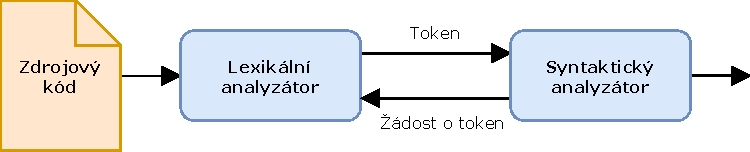
\includegraphics[width=1\textwidth]{img/lexicalAnalysis.pdf}
						\caption[lexicalAnalysis]{Princip lexikální analýzy}
						\label{lexicalAnalysis}
					\endminipage\hfill
				\end{figure}			
			
		\subsection{Syntaktická analýza}
			Ve chvíli, kdy je text převeden do lexémů pomocí lexikální analýzy, je možné provést syntaktickou analýzu, někdy nazývanou parsování. Lexikální analýza není schopna kontrolovat syntaxi kvůli limitacím regulárních výrazů. Syntaktická analýza však pracuje na úrovni bezkontextové gramatiky, která je té regulární nadřazená, proto to umožňuje. Na obrázku \ref{bkg} je možné vidět ukázku této gramatiky. Velká písmena (\texttt{S}, \texttt{Z}, \texttt{E}, ..) představují neterminální symboly, jejichž výčet je na levé straně obrázku. Za šipkou pak následuje, na co je možné dané neterminální symbol přepsat. To často mohou být další neterminální symboly a celý výraz se takto rozrůstá. Svislými čarami (\texttt{|}) jsou odděleny možnosti, na které se může symbol přepsat. Symbol \texttt{F} tedy může být rozepsán na \texttt{(E)} nebo na \texttt{V}.\\
			
			Ostatní řetězce (zde \texttt{if}, \texttt{then}, \texttt{\{}, ...) jsou potom terminální výrazy, které jsou konečné a nejde je dále rozepsat. Symbol malé \texttt{e} je speciální a představuje prázdný znak, který ukončuje danou posloupnost. Pomocí symbolů \texttt{+} a \texttt{*} je možné vyjádřit opakování daného výrazu. Tímto způsobem je tedy možné vyjádřit gramatiku programovacího jazyka. Pokud vstupní lexémy neodpovídají této gramatice, vzniká syntaktická chyba.
			
			\begin{figure}[!htb]
				\minipage{1\textwidth}	
					\centering
					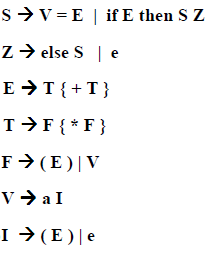
\includegraphics{img/gramatika.png}
					\caption[bkg]{Ukázka bezkontextové gramatiky}
					\label{bkg}
				\endminipage\hfill
			\end{figure}
			
			Jedním ze způsobů, jak zpracovávat tuto gramatiku je rekurzivní sestup. Každý z neterminálních symbolů je prezentován procedurou, která se vykoná, ve chvíli, kdy se jedná o daný symbol. Takto se postupně rekurzivně volají procedury dokud není zpracován celý vstup. V proceduře s terminálním souborem pak můžeme vykonat určitou akci, která koresponduje s~daným výrazem, např. přidat do seznamu další strojovou instrukci. Pro rozhodování je použita technika, kdy se nahlíží na další lexémy na vstupu a podle toho se určí o jaký výraz se jedná. Gramatika musí být vždy jednoznačná.
			
		\subsection{Nástroje}
			I přesto, že by bylo možné provádět zmíněné analýzy pomocí vlastního kódu, je také možné použít některý z dostupných nástrojů. Tyto nástroje umožňují parsování zdrojového kódu za použití samostatné aplikace nebo se může jednat o knihovnu, jejíž API můžeme použít přímo v našem kódu.
			
			\paragraph{JFLex}
				JFLex \cite{jflex} je lexikální analyzátor pro jazyk Java. Protože lexikální analýza sama o sobě nestačí k analýze kódu vhodné pro detekci kontraktů, je třeba tento nástroj použít s jiným, který umožní syntaktickou analýzu. Může se jednat např. o ANTLR, BYacc/J či CUP. 						
						
			\paragraph{ANTLR}			
				ANTLR \cite{antlr} je široce používaný nástroj, který umožňuje na základě zadané gramatiky vytvořit a procházet strom daného zdrojového kódu. ANTLR je primárně určen ke zpracování vlastní gramatiky např. při tvorbě vlastního překladače, nicméně je možné také použít gramatiku jazyka Java pro rozbor jejího zdrojového kódu.
			
			\paragraph{JavaParser}
				JavaParser \cite{javaparser} je jedním z dostupných nástrojů, který umožňuje analýzu, parsování ale i konstruování kódu jazyka Java. Funguje jako knihovna, kterou můžeme použít v našem kódu. Jedná se o vyspělou technologii, která je použita v řadě projektů. 
				
			\paragraph{Roaster}
				Roaster \cite{roaster} je nástroj podobný JavaParser. Také umožňuje nejen parsování, ale i editaci zdrojových kódů jazyka Java. Mimo dostupného API umožňuje také práci s konzolí  pro jednoduché použití.
	

	\section{Gramatika jazyka Java}
		Vzhledem k tomu, že Java je plnohodnotný programovací jazyk s řadou funkcí, je jeho specifikace gramatiky \cite{javaGrammar} velice rozsáhlá. V této části budou pouze vyzdviženy některé informace, které mohou být důležité pro problematiku extrakce kontraktů. Tyto informace budou vycházet ze specifikace Java verze 1.8, nicméně by měly být shodné i s ostatními verzemi současné doby.\\
		
		Java je definována dvěma bezkontextovými gramatikami. Jedna z nich je lexikální a ta specifikuje, jak vypadají jednotlivé lexémy. Určuje, co může obsahovat identifikátor, jaká jsou klíčová slova, omezovače atd. Této části zde nebude věnována velká pozornost. Naopak druhou gramatikou, která je z hlediska extrakce kontraktů důležitější, je syntaktická gramatika.
		 
		\subsection{Syntaxe}
			Syntaxe určuje, jaké posloupnosti lexémů jsou povolené pro správně fungující program. Protože se stále jedná o gramatiku, bude se při popisu vycházet z~toho, že se daný úsek vždy skládá z neterminálů, které se přepisují na terminály a neterminály. Terminály (např. \texttt{\textcolor{pblue}{class}}) jsou konečné prvky, které není dále možné rozvíjet, zatímco neterminály (např. \texttt{ClassModifier}) zastupují jiné neterminály a terminály. Neterminál uzavřený v hranatých závorkách (\texttt{[]}) se může vyskytnou nejvýše jedenkrát. Složené závorky (\texttt{\{\}}) pak určují, že se daný neterminál může vyskytnout nejvýše n-krát. Pravá strana rozdělená do více řádek je pouze příliš dlouhá než aby se na daný řádek vešla. Nejedná se alternativní možnost přepisu. Ty jsou vždy rozděleny symbolem svislé čáry (\texttt{|}).
			
			\subsubsection{Kompilační jednotka}	
				Výchozím bodem je tzv. \emph{compilation unit}, nebo-li kompilační jednotka. Z~hlediska gramatiky se jedná o nejobecnější neterminál, jinak řečeno počáteční symbol, ze kterého vycházejí všechny ostatní neterminály. V praxi se jedná o zdrojový soubor jazyka Java.\\\\
				\- \- \- \- \- \- \texttt{CompilationUnit $\rightarrow$}\\
				\- \- \- \- \- \- \- \- \- \- \- \- \texttt{[PackageDeclaration] \{ImportDeclaration\} \{TypeDeclaration\}}\\
				
				Zde je vidět, že se kompilační jednotka skládá z deklarace balíčku, deklarace importů a deklarace typu. Deklarace balíčku je jedna volitelná položka, kterou lze použít ke specifikaci toho, v jakém balíčku se tento soubor nachází. Neterminál \texttt{ImportDeclaration} představuje importy, kterých může být libovolné množství. Symbol \texttt{TypeDeclaration} pak představuje deklaraci rozhraní nebo deklaraci třídy. Samotná deklarace třídy se pak ještě dělí na deklaraci výčtového typu a deklaraci běžné třídy.
			
			\subsubsection{Deklarace třídy}
				Třídy představují základní stavební jednotku objektového jazyka Java. Z~hlediska syntaxe zde bude popsána deklarace běžné třídy, nicméně deklarace rozhraní a výčtového typu jsou v mnoha ohledech podobné.\\\\
				\- \- \- \- \- \- \texttt{NormalClassDeclaration $\rightarrow$}\\
				\- \- \- \- \- \- \- \- \- \- \- \- \texttt{\{ClassModifier\} \textcolor{pblue}{class} Identifier [TypeParameters]}\\  	 
				\- \- \- \- \- \- \- \- \- \- \- \- \texttt{[Superclass] [Superinterfaces] ClassBody}\\
	
				Neterminál \texttt{ClassModifier} zde představuje modifikátor třídy. Mohou zde být definovány anotace (viz níže) a také určení, zda je daná třída veřejná či privátní, zda je abstraktní, statická atd. Symbol \texttt{Identifier} reprezentuje identifikátor nebo-li pojmenování dané třídy. To musí být unikátní jinak nastává kompilační chyba. \texttt{TypeParameters} představuje typové určení ve špičatých závorkách (např. \texttt{List<String>}). V případě \texttt{Superclass} se pak jedná o dědičnost (tedy \texttt{extendes NAZEV}) a \texttt{Superinterfaces} zastupuje implementace rozhraní (tedy \texttt{implements NAZEV}). Položka \texttt{ClassBody} představuje celé tělo třídy, jsou tu tedy atributy, konstruktory, metody atd.	 
		 
			\subsubsection{Deklarace metody}
				Metoda se z hlediska gramatiky skládá ze tří složek. Nejprve jsou zde modifikátory metody \texttt{MethodModifier}. Jedná se o stejné položky jako v případě třídy, tedy anotace a definice \texttt{private/protected/public}, \texttt{static}, \texttt{final} atd. Neterminál \texttt{MethodHeader} představuje hlavičku metody, ta je podrobněji popsána dále. Poslední částí je \texttt{MethodBody}, tedy tělo metody. To se skládá z bloku kódu, který je z hlediska syntaxe velice komplexní. Jsou zde podmínky, cykly, volání metod, definice proměnných atd.\\\\
				\- \- \- \- \- \- \texttt{MethodDeclaration $\rightarrow$}\\
				\- \- \- \- \- \- \- \- \- \- \- \- \texttt{\{MethodModifier\} MethodHeader MethodBody}\\\\
 				\- \- \- \- \- \- \texttt{MethodHeader $\rightarrow$}\\
				\- \- \- \- \- \- \- \- \- \- \- \- \texttt{Result MethodDeclarator [Throws]}\\\\
				\- \- \- \- \- \- \texttt{MethodDeclarator $\rightarrow$}\\
				\- \- \- \- \- \- \- \- \- \- \- \- \texttt{Identifier ( [FormalParameterList] ) [Dims]}\\

				Hlavička metody tvoří hlavní část její signatury. Symbol \texttt{Result} představuje návratový typ metody. \texttt{Throws} umožňuje propagaci výjimek pomocí klíčového slova \texttt{throws}. Neterminál \texttt{MethodDeclarator} se pak dále člení. \texttt{Identifier} opět představuje identifikátor, tedy jméno dané metody. V závorce jsou pak uvedeny jednotlivé parametry. Ty se typicky skládají z definice typu a identifikátoru. Volitelné jsou pak opět různé modifikátory včetně anotací.	
 		
			\subsubsection{Deklarace anotace} 
				Běžné anotace jsou definovány pouze symbolem \texttt{@} následovaným názvem anotace. Poté je možné volitelně do závorek uvést další parametry. Symbol \texttt{TypeName} reprezentuje název, ten musí představovat validní anotaci, jinak nastane chyba. Za názvem s v závorce mohou nacházet další parametry. Neterminál \texttt{ElementValue} představuje jednu položku hodnoty anotace. Může se jednat o libovolný objekt, pole, další anotaci, ternární výraz atd. \texttt{ElementValuePairList} pak představuje seznam přiřazení typu: \texttt{identifikátor = hodnota}.\\\\\\
				\- \- \- \- \- \- \texttt{Annotation $\rightarrow$}\\
				\- \- \- \- \- \- \- \- \- \- \- \- \texttt{\textcolor{pblue}{@} TypeName |}\\
				\- \- \- \- \- \- \- \- \- \- \- \- \texttt{\textcolor{pblue}{@} TypeName ( ElementValue ) |}\\
				\- \- \- \- \- \- \- \- \- \- \- \- \texttt{\textcolor{pblue}{@} TypeName ( [ElementValuePairList] )}\\		
	
	\section{Retenční politika anotací}		
				\emph{Retention Policy} \cite{retentionPolicy}, nebo-li retenční politika, určuje, v jaké chvíli mají být anotace odebrány z programu. V Java existují tři typy retenčních politik, jsou uchovány ve výčtovém typu \texttt{java.lang.annotation.RetentionPolicy}: 
					
					\begin{itemize}
						\item \texttt{SOURCE}
						\item \texttt{CLASS}
						\item \texttt{RUNTIME}
					\end{itemize}
					
				Anotace s retenční politikou \texttt{SOURCE} bude uchována pouze ve zdrojovém kódu a během kompilace bude zahozena. Politika \texttt{CLASS} říká, že anotace zůstane zachována během kompilace, ale je zahozena při běhu programu. Retenční politika \texttt{RUNTIME} pak zajišťuje, že bude anotace dostupná i při běhu programu. Výchozí hodnotou je \texttt{CLASS}. To je možné změnit při definici dané anotace využitím jiné anotace \texttt{@Retention}. To je možné vidět na příkladu níže.\\\\
				\- \- \- \- \- \- \texttt{@Retention(RetentionPolicy.RUNTIME)}\\
				\- \- \- \- \- \- \texttt{public @interface MySampleAnnotation \{}\\
				\- \- \- \- \- \- \- \- \- \texttt{...}\\
				\- \- \- \- \- \- \texttt{\}}\\

				Pokud nemají anotace retenční politiku \texttt{SOURCE}, jsou také zaneseny do bajtkódu. Jedná se tedy o podmínkou proto, abychom mohli extrahovat kontrakty definované anotacemi z přeložených souborů. Např. anotace reprezentací JSR305 mají retenční politiku \texttt{RUNTIME} a jsou tedy uchovány v~bajtkódu.
	
	\section{Rozbor přeložených souborů}
		Při analýze kontraktů v jiných projektech není vždy možné získat zdrojové soubory. Z toho důvodu je užitečné umět analyzovat nejen soubory \texttt{.java}, ale také přeložené soubory \texttt{.class}.
	
		\subsection{Dekompilace}
			Aby bylo možné soubory analyzovat, musíme je nejprve dekompilovat. Dekompilace je vlastně opačný proces kompilace a jejím cílem je tedy získat původní zdrojový kód z cílové podoby. Tou bývají obvykle strojové instrukce, v případě Java se jedná o bajtkód. Výhodou bajtkódu je, že obsahuje vysoké množství různých podrobností, které umožňují téměř bezztrátovou rekonstrukci zdrojového kódu. Jednoduchý princip je vidět na obrázku \ref{decompilation}.
			
			\begin{figure}[!htb]
				\minipage{1\textwidth}	
					\centering
					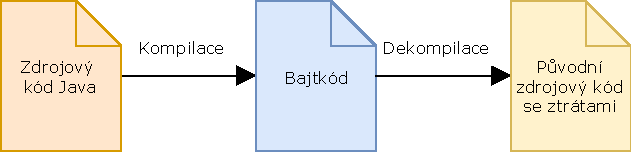
\includegraphics{img/decompilation.pdf}
					\caption[decompilation]{Dekompilace}
					\label{decompilation}
				\endminipage\hfill
			\end{figure}
			
			\subsubsection{Nástroje}
				Nástrojů pro dekompilaci souborů v jazyce Java je celá řada. Některé je nutné pouštět samostatně, ty pak mohou být vytvořeny i v jiných programovacích jazycích. Vývojová prostředí jako např. Eclipse či IDEA IntelliJ umožňují instalaci balíčků, které podporují dekompilaci souborů. Některé z~nástrojů je také možné použít přímo v kódu formou knihovny. Následuje seznam některých dostupných nástrojů, které jsou stále aktualizovány a umožňují dekompilaci moderních prvků jazyka Java \cite{top8decompilers}\cite{decompilersOnline}\cite{quickDecompilers}.	
				
				\paragraph{JD Project}
					JD Project (Java Decompiler) \cite{jd} je jedním z nejčastěji referovaných nástrojů v rámci Java dekompilace. JD disponuje samostatnou aplikací s grafickým uživatelským rozhraním, pomocí kterého je možné soubory dekompilovat a ihned vidět výsledek. JD také poskytuje doplněk do Eclipse a IDEA IntelliJ. Nejedná se o open-source nástroj, ale je dostupný zdroj pro GUI aplikaci. Nástroj bohužel nedisponuje API, aby bylo možné jej použít přímo v kódu.
					
				\paragraph{Procyon}
					Procyon \cite{procyon} je open-source nástroj, který také umožňuje dekompilaci. Nemá samostatné GUI jako JD, nicméně je možné reprezentaci zobrazit použitím externích nástrojů. Disponuje také API, které je možné použít přímo v kódu. Stačí zavolat metodu \texttt{decompile()}, kam vstupuje jméno souboru, který chceme dekompilovat a také kam má být směrován výstup. Výsledkem je pak zdrojový kód. Nejedná se samozřejmě přesnou kopii, ale jsou zde jisté limitace (viz níže).
					
				\paragraph{CFR}
					CFR \cite{cfr} je dalším z nástrojů, který umožňuje dekompilaci i konstrukcí Java 1.9. Nástroj je možné použít pouze v rámci příkazové řádky, kdy je na výstup směrován dekompilovaný kód. Součástí tedy není API, které by umožnilo použití v kódu.\\
					
				Nástrojů pro dekompilaci jazyka Java je velké množství a jejich výběr není snadný zejména poroto, že se neustále vyvíjejí na základě nových verzí Java. Při výběru je samozřejmě také důležité, jakým způsobem je daný nástroj možné používat, jaké konstrukce dokáže dekompilovat a roli může hrát také rychlost.
				
			\subsubsection{Rozdíly oproti původním souborům}
				Jak již bylo zmíněno, velice závisí na použitém nástroji pro dekompilaci. Jestliže daný nástroj nepodporuje určité konstrukce, pak je logické že jejich dekompilace nebude možná a není tak možné získat původní zdrojový soubor. Pokud nástroj umožňuje dekompilaci všech použitých konstrukcí, výsledný kód stále nebude zcela shodný. Přeložený kód obsahuje plné cesty k objektům, doplňuje neuvedená přetypování atd. Tyto informace často ve zdrojových kódech nebývají uvedené, protože jsou redundantní, ale při rekonstrukci přeloženého souboru není možné určit, kde tyto informace byly a~kde ne. Přirozeně také není možné získat data, která se do bajtkódu nezanášejí, jako jsou např. komentáře.

% Datový model
\chapter{Datový model}
	Tato kapitola se zabývá podrobnostmi o datovém modelu. Pojednává o volbě reprezentace kontraktů, které byly použity pro tento projekt a obecně o~společných atributech kontraktů. Jsou zde uvedeny podrobnosti o datovém modelu určeném pro reprezentaci kontraktů, ale také pro výsledky jejich porovnání. Oba tyto modely jsou zde popsány slovně, ale i pomocí UML diagramu. Závěr tvoří informace o externí reprezentaci těchto dat.

	\section{Volba DbC konstrukcí}
		Po analýze dostupných materiálů jsem se rozhodl zvolit pro implementaci konstrukce Guava Preconditions a JSR305. Důvodem byla především jejich rozdílná reprezentace, kdy Guava Preconditions je realizováno pomocí volání metod uvnitř těl metod, tedy se jedná o knihovnu, která zprostředkovává API. Avšak Guava Preconditions umožňuje tvorbu pouze vstupních podmínek.\\
		
		 Na druhé straně JSR305 je tvořené anotacemi v záhlaví tříd, metod a~také jako součást parametrů metod. Umožňuje tvoření všech tří typů kontraktů (vstupní, výstupní i neměnné podmínky). Kromě této diverzity se také jedná o jedny z častých konstrukcí používaných v projektech viz \cite{contractsInWild}. Principy obou těchto nástrojů byly již popsány výše (viz kapitola 3 - Popis kontraktů softwarových rozhraní), z čehož se bude vycházet.
				
				
	\section{Společné znaky reprezentací kontraktů}		
		Při rozboru jednotlivých nástrojů pro reprezentaci design by contract zjistíme, že sdílejí mnoho podobných aspektů, které jsou klíčové pro vytvoření obecného modelu, který je schopen zachytit libovolnou konstrukci kontraktu.\\ 
		
		Do modelu je třeba nejprve zanést, o jaký nástroj pro práci s kontrakty se jedná (Guava, JSR305, atd.). Každý kontrakt je také vždy definován jedním ze tří typů podmínek (vstupní, výstupní a neměnná), to je také velmi důležitá informace, kterou je třeba do modelu zaznamenat. Kontrakty jsou také typicky definovány funkcí, která určuje, co kontrakt ověřuje. Může se jednat o kontrolu argumentu, zda objekt není \texttt{null} atp. V případě, že kontrakt tuto informaci neobsahuje, může tato položka zůstat prázdná.\\
		
		Další důležitou informací je hodnota daného kontraktu, která představuje výraz, který je vyhodnocován. Některé kontrakty tuto hodnotu nevyžadují (např. \texttt{@Nonnull} u JSR305), ale ve většině případů jde o podmínku (např. \texttt{x~> 0}). Některé druhy reprezentací kontraktů však umožňují i další argumenty. Typicky se jedná o informace o typu výjimky, která je vyhozena, či o~její zprávě. Může se však také jednat o další upřesňující data. Obvykle tyto informace nemají z hlediska důležitosti vysokou prioritu, přesto by ale mělo být možné je do modelu zahrnout.
		
	
	\section{Model pro extrakci kontraktů}
			Aby bylo možné kontrakty extrahovat ze zdrojových souborů, je také třeba mít k dispozici datový model, do kterého bude možné tato data uložit. Tento model jsem vytvořil na základě analýzy konstrukcí kontraktů s ohledem na následný export do formátu dat, který bude možné dále zpracovávat. Aby byl zachován kontext kontraktů, usoudil jsem, že bude třeba ukládat také informace o třídách a metodách v daném souboru.\\
			
			Rozhodl jsem se tedy vytvořit strukturu podobnou stromu, jejíž kořenem je samotný zdrojový soubor (třída \texttt{JavaFile}). Tento soubor obsahuje různé podrobnosti o tomto souboru jako je jeho jméno a cesta, typ a statistiky o~jeho obsahu. Také obsahuje seznam všech tříd (třída \texttt{JavaClass}) obsažených v tomto souboru.\\
			
			Každá jednotlivá třída pak obsahuje jméno, svou hlavičku, seznam metod (třída \texttt{JavaMethod}) a také seznam všech kontraktů týkajících se této třídy, tedy neměnných podmínek. Metoda pak nese informaci o své signatuře a~také seznam všech kontraktů (třída \texttt{Contract}) dané metody. Samotný kontrakt pak obsahuje informaci o tom, o jaký typ kontraktu a podmínky se jedná, kompletní výraz a také jeho dílčí části (viz podrobnosti níže).\\
			
			V projektu je model reprezentován v rámci knihovny nástroje. Je zde balíček \texttt{model}, kde se nacházejí všechny zmíněné třídy.\\
			
			Na obrázku \ref{modelExtractorDiagram} je vidět grafické znázornění datového modelu formou UML diagramu. Nejsou zde záměrně zobrazeny objekty \texttt{ContractComparison} a \texttt{JavaFileCompareReport}. Těm je věnován prostor v diagramu pro porovnávání kontraktů, který je na obrázku \ref{modelComparatorDiagram}.\\ 
							
				\begin{figure}[!htb]
					\minipage{1\textwidth}	
						\centering
						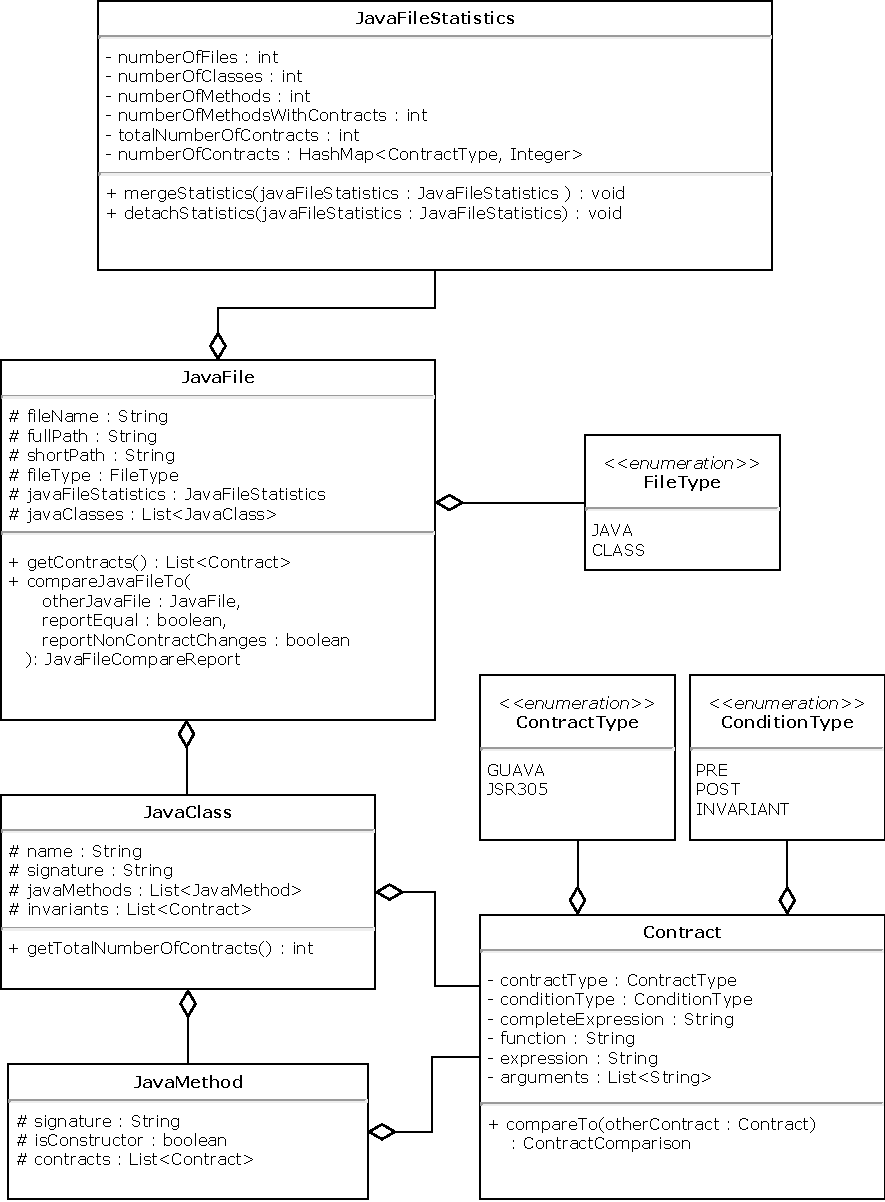
\includegraphics[width=1\textwidth]{img/modelExtractorDiagram.pdf}
						\caption[modelExtractorDiagram]{UML diagram datového modelu pro extrakci kontraktů}
						\label{modelExtractorDiagram}
					\endminipage\hfill
				\end{figure}				
			
			\subsection{Podrobnosti modelu}
				Následuje rozbor některých prvků modelu, které nemusejí být na první pohled samovysvětlující či je vhodné je vyzdvihnout kvůli své důležitosti.
				
				\subsubsection{Atribut \texttt{shortPath}}				
					Atribut \texttt{shortPath} ve třídě \texttt{JavaFile} slouží k zobrazení zkrácené cesty souboru, což zlepšuje přehlednost uživatelské aplikace. Pokud jsou přidány soubory ze stejné složky, které jsou hluboko v hierarchii souborového systému, název souboru by mohl být příliš dlouhý, aniž by poskytoval užitečnou informaci.\\
					
					Např. místo toho, aby byl soubor reprezentován dlouhou absolutní cestou \texttt{C:/test/guava-10.0/com/google/common/base/Objects.java}, zobrazí se pouze \texttt{base/Objects.java}. Jiný soubor pak může být reprezentován např. pomocí \texttt{util/concurrent/Atomics.java}. Zkrácená cesta se průběžně mění na základě přítomných souborů, aby bylo vždy možné je jednoznačně rozeznat. V případě potřeby, či aktualizace této cesty, je k dispozici absolutní cesta v atributu \texttt{fullPath}.
				
				\subsubsection{Třída \texttt{JavaFileStatistics}} 
					Atribut \texttt{totalNumberOfContracts} obsahuje informaci o celkovém počtu kontraktů nehledě na typ reprezentace. Naopak hash mapa \texttt{numberOfContracts} poskytuje celkový počet kontraktů pro daný typ reprezentace.\\
				
				Metody \texttt{mergeStatistics()} a \texttt{detachStatistics()} slouží ke sloučení respektive odloučení dané statistiky od aktivní statistiky. Tyto metody jsou využity při kalkulaci globálních statistik, kde je nutné provést aktualizaci vždy po přidání resp. odebrání souborů.
					
				
				\subsubsection{Třída \texttt{Contract}}	
					Klíčovou částí celého modelu je jednoznačně třída \texttt{Contract}. Instance této třídy představují jednotlivé kontrakty souboru. Kontraktem je zde myšlena jedna vstupní, výstupní či neměnná podmínka doprovázena dalšími atributy. Následuje krátký popis a vysvětlení jednotlivých atributů této třídy.
					
					\paragraph{\texttt{ContractType contractType}} 
						Jedná se o výčtový typ, který určuje o jaký druh kontraktu se jedná. Při současném stavu knihovny to mohou být hodnoty Guava či JSR305.
			
					\paragraph{\texttt{ConditionType conditionType}} 
						Opět výčtový typ, který určuje typ kontraktu dle jeho podmínky. Rozlišují se tři druhy: \texttt{PRE} pro vstupní podmínku, \texttt{POST} pro výstupní podmínku a \texttt{INVARIANT} pro neměnnou podmínku.
			
					\paragraph{\texttt{String completeExpression}} 
						Reprezentuje kompletní výraz celého kontraktu. I přesto, že celý výraz je možné vytvořit z jeho dílčích částí, je zde uveden pro rychlý přehled. Může také posloužit jako kontrola parsování či pro rychlé porovnání.
			
					\paragraph{\texttt{String function}} 
						Tento řetězec určuje funkci, o jakou se jedná v rámci daného kontraktu. V případě Guava se jedná o název metody, v případě JSR305 o název anotace. Obecně se jedná o hlavní označení určující daný kontrakt.
			
					\paragraph{\texttt{String expression}} 
						Obsahuje první parametr dané funkce. Důvodem, proč oddělit první parametr od ostatních, bylo, že kontrakty mají často pouze jeden parametr a pokud jich mají více, ostatní často nejsou tolik relevantní. Pro zvýšení přehlednosti byl tedy tento parametr uveden samostatně.
			
					\paragraph{\texttt{List<String> arguments}} 
						Seznam ostatních argumentů daného kontraktu. Ostatní atributy až na výjimky slouží pouze k uvedení chybové zprávy, která se má zobrazit při porušení kontraktu. Mimo samotné zprávy zde také často bývají proměnné použité v šabloně zprávy.
					
				\subsubsection{Další třídy} 
					Během zpracování byly také používány následující třídy: \texttt{ExtendedJavaFile}, \texttt{ExtendedJavaClass} a \texttt{ExtendedJavaMethod}. Ty obsahují dodatečné informace vůči svým protějškům ve výše zmíněném modelu. Navíc obsahují informace o anotacích, vstupních parametrech a jednotlivých částech těl metod. Po zpracování jsou pak tyto objekty redukovány na ty výše zmíněné, které jsou připraveny pro externí reprezentaci.
		

	\section{Model pro porovnávání kontraktů}
		Vzhledem k tomu, že cílem nástroje nebyla pouze extrakce kontraktů, ale také jejich případné porovnání, bylo třeba vytvořit datový model, který umožní zachytit i tyto informace. Model jsem navrhoval s vědomím, že porovnání bude mít největší hodnotu ve chvíli, kdy bude možné porovnat kontrakty dvou projektů, tedy dvou složek. Samozřejmě nemá velký smysl porovnávat kontrakty dvou naprosto rozdílných projektů. Myšlenkou je porovnání dvou různých verzí téhož projektu. Pak je možné pozorovat, zda kontrakty přibývají či ubývají s rostoucím množstvím kódu a obecně různé trendy, které mohou poskytnout zajímavé informace o této problematice.\\ 
		
		S porovnáním dvou složek však také přibývá problém párování jednotlivých souborů, tříd, metod a kontraktů se svými protějšky v druhé složce. Na základě těchto informací jsem se tedy rozhodl, že hlavním objektem pro porovnání bude zpráva o rozdílech těchto dvou složek (projektů). Tato zpráva bude obsahovat různé podrobnosti o tom, zda byly složky shodné, konkrétní případy, kde se lišily a také seznam souborů, ke kterým nebyl nalezen adekvátní pár v druhé složce. Tím vzniká tedy seznam přidaných respektive odebraných souborů podobně jako u porovnávání dvou verzí při práci s VCS\footnote{VSC, neboli Version Control System je druh nástroje, který umožňuje týmu spravovat kód v průběhu času.}. Stejně jako v případě extrakce, i zde je souhrn statistik, který poskytuje dodatečné informace o tomto srovnání.\\
				
		Porovnání jednotlivých souborů jsou pak zachycena v objektu, který má podobné atributy jako ten pro složku, tedy v čem se dané soubory lišili z~hlediska tříd, metod a zejména kontraktů. I zde je k dispozici souhrn statistik. Model by měl být patrný z z obrázku \ref{modelComparatorDiagram}, kde je znázorněn graficky formou UML diagramu. Následuje také popis některých částí modelu, které nemusejí být na první pohled jasné, či se jedná o důležité prvky.\\
		
		V projektu je pak tento model opět součástí knihovny a nachází se v~balíčku pro porovnávání (\texttt{comparator.comparatormodel}).
		
				\subsection{Podrobnosti modelu}
				
					\subsubsection{Atributy \texttt{apiEqual} a \texttt{contractEqual}}
						Tyto atributy určují, zda dvě složky či soubory jsou shodné z hlediska API respektive kontraktů. Atribut \texttt{apiEqual} tedy značí, zda jsou dané objekty shodné z hlediska definice tříd a jejich metod. Pokud například jeden soubor obsahuje metodu, kterou ten druhý nemá, či ji obsahuje, ale má pozměněnou signaturu, hodnotou \texttt{apiEqual} by bylo \texttt{false}.\\
						
						Atribut \texttt{contractEqual} značí, zda jsou dané objekty shodné z hlediska kontraktů. Tedy jestli jich obsahují stejný počet a zda jsou jednotlivé kontrakty shodné.
		
					\subsubsection{Třída \texttt{ApiChange}}
						Pomocí instancí této třídy je možné vyjádřit změny v API. Atribut \texttt{apiType} určuje, zda se změna týká třídy či metody. \texttt{apiState} pak určuje, zda byl daný element přidán, odebrán či tzv. \texttt{FOUND\_PAIR}. V tom případě se nejedná o změnu, ale naopak byl nalezen protějšek daného objektu. Pomocí instancí této třídy je pak vyjádřeno, které metody a třídy chybějí či se naopak nově objevily.
						
					\subsubsection{Třída \texttt{ContractComparison}}
						Tento výčtový typ představuje výsledek po porovnání dvou kontraktů. Může obsahovat tyto hodnoty:
						
						\paragraph{\texttt{EQUAL}}
							Tento výsledek značí, že jsou oba kontrakty naprosto shodné.
						
						\paragraph{\texttt{MINOR\_CHANGE}}
							Tento stav značí, že kontrakty jsou shodné, ale liší se v~ostatních argumentech. Typicky se jedná o změnu zprávy o chybě či různá upřesnění. Z tohoto důvodu se jedná o \emph{minor change} (menší změnu).
							
						\paragraph{\texttt{SPECIALIZED}}
							Tímto tvarem je možné vyjádřit, že daný kontrakt je shodný jako ten druhý, nicméně má přísnější podmínku, je tedy více specializovaný. Triviálním příkladem může být situace, kdy první kontrakt má podmínku \texttt{x >= 0} a ten druhý podmínku \texttt{x > 0}. Zde je vidět, že druhá podmínka je přísnější. V současném stavu nástroje není tato hodnota používána, byla však připravena pro budoucí rozšíření.
							
						\paragraph{\texttt{GENERALIZED}}
							Jedná se o stejnou hodnotu jako \texttt{SPECIALIZED} s tím rozdílem, že je kontrakt naopak více obecný a má tedy mírnější podmínku. Stejně ani tento stav není momentálně využit.
							
						\paragraph{\texttt{DIFFERENT\_EXPRESSION}}
							Tímto stavem je vyjádřeno, že jsou dané kontrakty typově shodné, liší se však v atributu \texttt{expression}. Obvykle tedy platí, že se liší v podmínce, či v objektu, kterého se daný kontrakt týká. V současném stavu tento stav zahrnuje také stavy \texttt{SPECIALIZED} i \texttt{GENERALIZED}. Do budoucna by však stav \texttt{DIFFERENT\_EXPRESSION} měl být přípustný pouze pokud ani z dvou zmíněných stavů není možné prokázat (např. podmínku \texttt{y~== 1} nelze porovnávat s podmínkou \texttt{x > 0}).
							
						\paragraph{\texttt{DIFFERENT}}
							Tento výsledek říká, že se oba kontrakty liší v některém ze základních atributů, tedy typ kontraktu či podmínky. Při porovnávání dvou souborů či složek by nemělo být možné tohoto stavu docílit, protože není možné nalézt pár k danému kontraktu, jestliže se takto výrazně liší. Důvodem tohoto stavu je zajištění úplnosti v případě porovnávání dvou kontraktů bez známého kontextu. 						 
							
		
				\begin{figure}[!htb]
					\minipage{1\textwidth}	
						\centering
						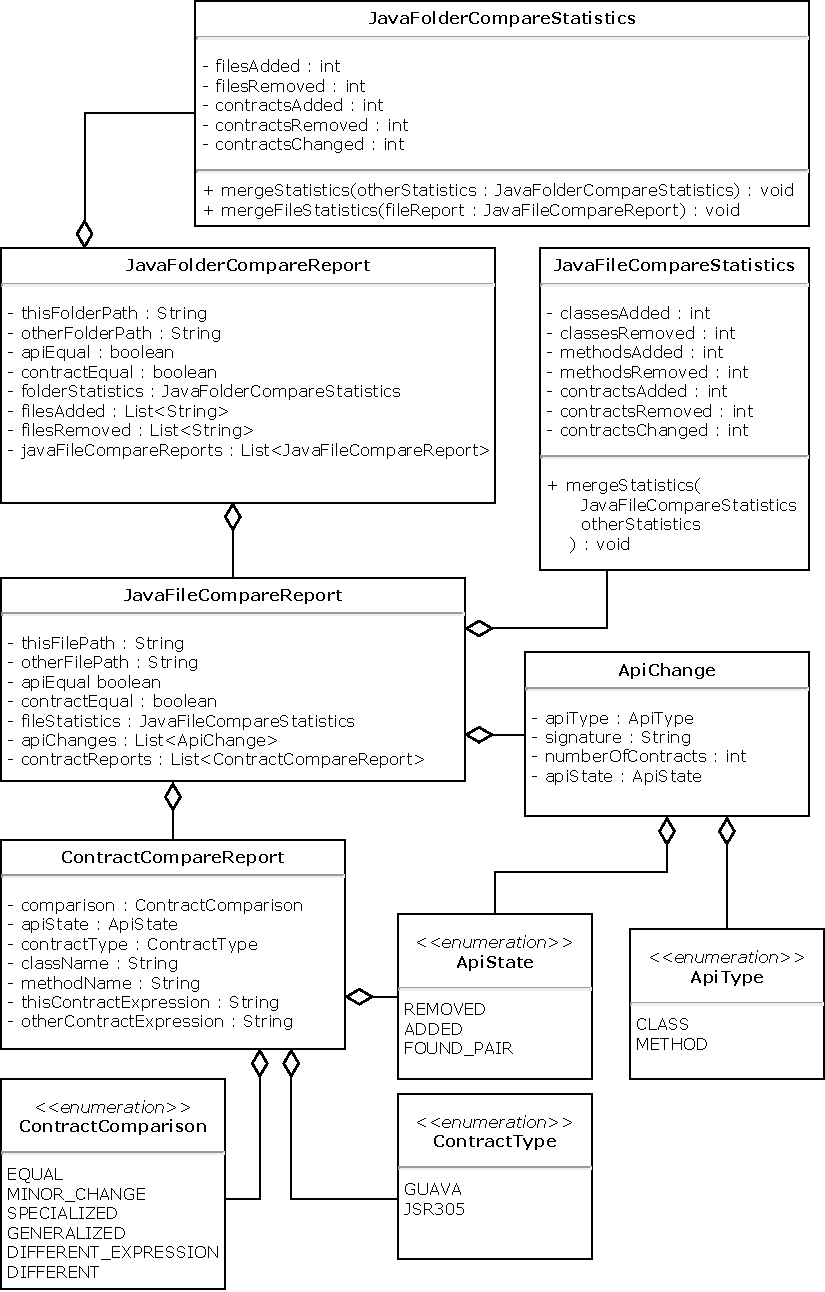
\includegraphics[width=1\textwidth]{img/modelComparatorDiagram.pdf}
						\caption[modelComparatorDiagram]{UML diagram datového modelu pro porovnání kontraktů}
						\label{modelComparatorDiagram}
					\endminipage\hfill
				\end{figure}

			
	\section{Externí reprezentace modelu}
		Pro externí reprezentaci modelu jsem zvolil použití formátu JSON. Tento formát je široce používaný zápis dat a umožňuje relativně snadné ukládaní objektů typu Java. JSON je tak vhodný pro zpracovaní strojem, ale je dobře čitelný i pro lidské oko (v případě, že byl zformátován). Díky těmto kvalitám je JSON vhodným formátem pro zobrazení, archivaci i další zpracování extrahovaných dat.\\
			
			Alternativou bylo použití formátu XML. Tento formát má v podstatě stejné přednosti jako JSON, s tím rozdílem, že obvykle není potřeba dalšího formátování proto, aby byl čitelný pro člověka, nicméně je oproti formátu JSON více opsaný. I přesto, že XML by byla také validní možnost pro reprezentaci dat, po dohodě s vedoucím práce jsme se rozhodli pro použití JSON. Důvodem byla zejména jeho stručnost, ale také lepší vlastnosti pro předávání mezi jinými nástroji.
			
		\subsection{Specifikace formátu}
			Formát JSON \cite{jsonSyntax} je velice jednoduchý a stručný. Objekty reprezentované v~JSON jsou uzavřeny ve složených závorkách (\texttt{\{\}}), jelikož celý soubor vždy představuje jeden komplexní objekt, daný soubor vždy začíná i končí složenou závorkou. Názvy dílčích atributů jsou pak uzavřeny v uvozovkách a za dvojtečkou následuje jejich hodnota. Více atributů je pak odděleno čárkami.\\
			
			Daný atribut může mít přirozeně různé typy hodnot. Řetězce jsou standardně uvnitř uvozovek, čísla a výrazy \texttt{true/false} jsou pak bez uvozovek. Hodnotou však může být i další objekt či pole. Pole je uzavřeno v hranatých závorkách (\texttt{[]}) a položky jsou odděleny čárkami. Pokud je pole prázdné, jsou zde pouze obě závorky bez obsahu.\\
			
			Formát exportovaných souborů přímo vychází z výše zmíněných modelů. Daný soubor obsahuje tedy všechny objekty uvedené v modelu a je pouze převeden do formátu JSON. V následujícím příkladu je ukázka formátu souboru, který je vytvořen po extrakci kontraktů. Příklad je úmyslně zkrácen, v atributu \texttt{javaMethods} by standardně byly jednotlivé metody a v každé z~daných metod pak případné kontrakty. Také by zde byly další atributy jako jsou statistiky, typ souboru atd.\\
							
			\noindent
			\- \- \- \texttt{\{}\\	
			\- \- \- \- \- \- \texttt{"fileName": "example.java", }\\
			\- \- \- \- \- \- \texttt{"fullPath": "C:/test/example.java", }\\ 
			\- \- \- \- \- \- \texttt{...}\\
			\- \- \- \- \- \- \texttt{"javaClasses": [}\\
			\- \- \- \- \- \- \- \- \- \texttt{\{}\\
			\- \- \- \- \- \- \- \- \- \- \- \- \texttt{"name": "Example"}\\
			\- \- \- \- \- \- \- \- \- \- \- \- \texttt{"signature": "public class Example"}\\
			\- \- \- \- \- \- \- \- \- \- \- \- \texttt{"javaMethods": [}\\
			\- \- \- \- \- \- \- \- \- \- \- \- \- \- \- \texttt{...}\\ 
			\- \- \- \- \- \- \- \- \- \- \- \- \texttt{],}\\
			\- \- \- \- \- \- \- \- \- \- \- \- \texttt{"invariants": []}\\
      		\- \- \- \- \- \- \- \- \- \texttt{\}}\\
      		\- \- \- \- \- \- \texttt{]}\\
      		\- \- \- \texttt{\}}\\			

% Implementace
\chapter{Nástroj pro analýzu kontraktů}
	Cílem práce z hlediska implementace bylo vytvořit nástroj, který by umožňoval získání dat podle výše navrženého modelu ze zdrojové či přeložené formy Java programu. Výsledná aplikace by pak měla umožnit vytvoření externí reprezentace dat a případně také porovnání DbC konstrukcí. Nástroj by měl být schopen zpracovat alespoň dva způsoby popisu DbC konstrukcí a měl by dovolovat snadné rozšíření pro další způsoby. S využitím tohoto nástroje by pak měla být vytvořena jednoduchá uživatelská aplikace, která by sloužila k načtení a zobrazení dat modelu.\\
	
	Smyslem aplikace je umožnit detekci kontraktů ve zdrojových, respektive přeložených, souborech jazyka Java. Nalezené kontrakty je pak možné analyzovat a zkoumat způsob a četnost použití jednotlivých typů v různých projektech. Aby bylo možno získaná data dále analyzovat, je zde také export do formátu JSON. Nástroj umožňuje porovnání dvou adresářů se soubory, což může být užitečné zejména při porovnání různých verzí projektu. Můžeme tak zjistit, zda se nezměnilo rozhraní či zda se zpřísnily podmínky kontraktů oproti předchozí verzi.\\
	
	Celý nástroj je rozdělen do dvou velkých částí. První z nich je knihovna, která poskytuje všechny potřebné metody pro práci se soubory jazyka Java, jejich analýzu a zpracování, extrakci kontraktů a jejich následné porovnání a export. Druhou částí je uživatelská aplikace, která využívá metod této knihovny a umožňuje její pohodlnou obsluhu. Tento vztah je znázorněn na stručném obrázku \ref{globalArchitecture}. Na obrázku \ref{componentDiagram} je pak vidět komponentový diagram, který obsahuje více podrobností.
					
	\begin{figure}[!htb]
		\minipage{1\textwidth}	
			\centering
			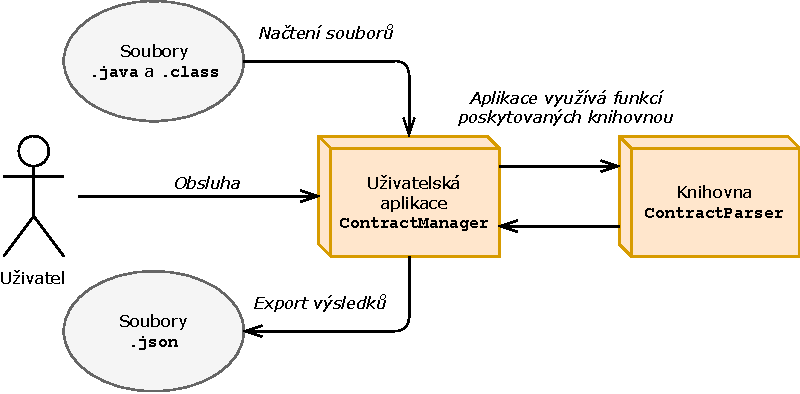
\includegraphics{img/globalArchitecture.pdf}
			\caption[globalArchitecture]{Architektura nástroje}
			\label{globalArchitecture}
		\endminipage\hfill
	\end{figure}
	
	\begin{figure}[!htb]
		\minipage{1\textwidth}	
			\centering
			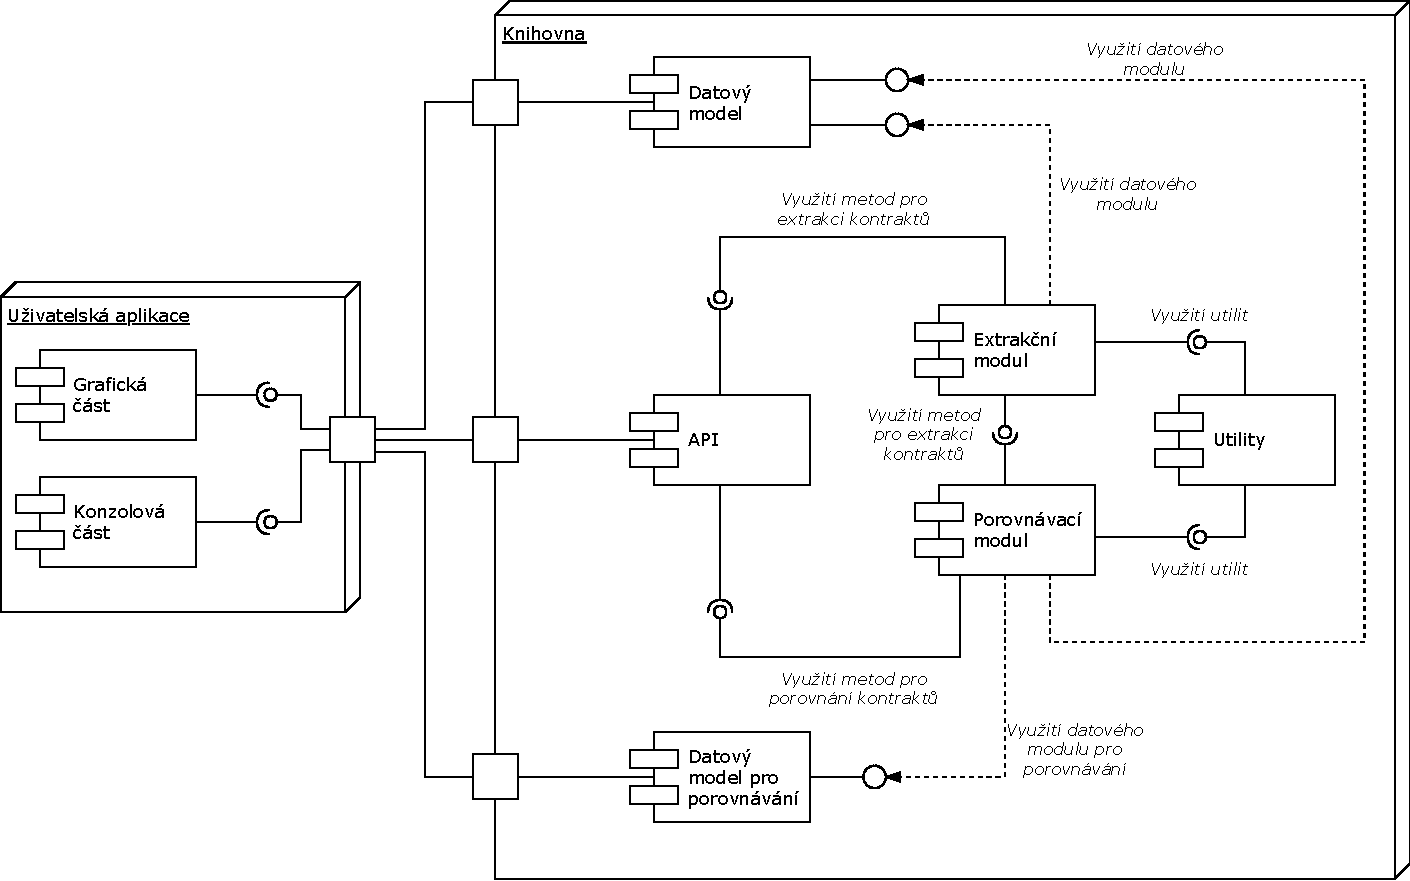
\includegraphics[width=1\textwidth]{img/componentDiagram.pdf}
			\caption[componentDiagram]{Komponentový diagram nástroje}
			\label{componentDiagram}
		\endminipage\hfill
	\end{figure}		
	
	% struktura projektu a potom v textu důležité třídy v implementaci + možná jejich uml model
	
%%%%%%%%%%%%%%%%%%%%%%%%%%%%%%%%%%%%%%%%%%%%%%%%%%%%%%%%%%%%%%%%%%%%%%%%%%%%%%%%%%%%%%%%%%%%%%%%%%%%%%%%%%%%%%%%%%%%%%%%%%%%%%%%%%%%%%%%%%%%%%%%%%%%%%%%%%%%%%%%%%%%%%%%%%%%%%%%%%%%%%%%
%%%%%%%%%%%%%%%%%%%%%%%%%%%%%%%%%%%%%%%%%%%%%%%%%%%%%%%%%%%%%%%%%%%%%%%%%%%%%%%%%%%%%%%%%%%%%%%%%%%%%%%%%%%%%%%%%%%%%%%%%%%%%%%%%%%%%%%%%%%%%%%%%%%%%%%%%%%%%%%%%%%%%%%%%%%%%%%%%%%%%%%%
%%%%%%%%%%%%%%%%%%%%%%%%%%%%%%%%%%%%%%%%%%%%%%%%%%%%%%%%%%%%%%%%%%%%%%%%%%%%%%%%%%%%%%%%%%%%%%%%%%%%%%%%%%%%%%%%%%%%%%%%%%%%%%%%%%%%%%%%%%%%%%%%%%%%%%%%%%%%%%%%%%%%%%%%%%%%%%%%%%%%%%%%
%%%%%%%%%%%%%%%%%%%%%%%%%%%%%%%%%%%%%%%%%%%%%%%%%%%%%%%%%%%%%%%%%%%%%%%%%%%%%%%%%%%%%%%%%%%%%%%%%%%%%%%%%%%%%%%%%%%%%%%%%%%%%%%%%%%%%%%%%%%%%%%%%%%%%%%%%%%%%%%%%%%%%%%%%%%%%%%%%%%%%%%%
	\section{Knihovna}
		Pro realizace nástroje jsem se rozhodl implementovat knihovnu, která poskytuje metody potřebné pro extrakci, porovnání a export kontraktů. Její součástí je také samozřejmě model použitý pro jejich reprezentaci. 

%%%%%%%%%%%%%%%%%%%%%%%%%%%%%%%%%%%%%%%%%%%%%%%%%%%%%%%%%%%%%%%%%%%%%%%%%%%%%%%%%%%%%%%%%%%%%%%%%%%%%%%%%%%%%%%%%%%%%%%%%%%%%%%%%%%%%%%%%%%%%%%%%%%%%%%%%%%%%%%%%%%%%%%%%%%%%%%%%%%%%%%%	
	    \subsection{Použité technologie}
	    
	    	\subsubsection{Programovací jazyk}
				Pro realizaci knihovny jsem použil jazyk Java verze 1.8. Jedním z hlavních důvodů bylo, že nástroj zkoumá reprezentace kontraktů v jazyce Java, díky tomu je možné dané konstrukce snadno testovat a zkoušet přímo v tomto projektu. Vedoucí práce také upřednostňoval použití jazyka Java z důvodů případného propojení s jinými nástroji, které byly vyvinuty pro práci s kontrakty v rámci univerzity a jsou také realizovány v Java. Osobně mám s jazykem Java pravděpodobně největší zkušenosti, což byl další z důvodů, proč tento jazyk použít. Z těchto důvodů byla volba jazyka poměrně jednoznačná.\\
				
				I přesto, že v průběhu vývoje projektu vyšla verze Java 1.9 a posléze i 1.10, rozhodl jsem se po domluvě s vedoucím práce ponechat stabilní verzi 1.8 a nepřecházet v průběhu vývoje na novější verzi jazyka.
				
			\subsubsection{Vývojové prostředí}				
				Nástroj byl realizován ve vývojovém prostředí IDEA IntelliJ Ultimate 2017.3.3.
	    	
			\subsubsection{Práce se závislostmi}
				Pro zajištění závislostí jako jsou knihovny třetích stran, ale také pro snadnou distribuci knihovny jsem zvolil technologii Apache Maven \cite{maven}. Jedná se o široce používaný nástroj pro získávání závislostí a tvorbu projektů.
				
			\subsubsection{Logování}
				Pro logování, tedy zobrazení a uložení chybových či informačních zpráv, byla použita knihovna Apache Log4j \cite{log4j}. Tato knihovna umožňuje pokročilé možnosti logování, které je možné dobře nastavit pomocí konfiguračních souborů. Opět se jedná o široce používanou technologii.
				
			\subsubsection{Tokenizace zdrojových souborů jazyka Java}
				Pro implementaci tokenizace souborů jsem se rozhodl použít knihovnu JavaParser \cite{javaparser}. Učinil jsem tak na základě mého průzkumu (viz 4. kapitola Tokenizace jazyka Java). Knihovna poskytuje komplexní reprezentaci daného zdrojového souboru a je tak možné jej dále analyzovat a zpracovávat. Knihovnu je možné snadno použít přímo v projektu díky zprostředkovanému API.
			
			\subsubsection{Dekompilace přeložených souborů jazyka Java}
				Jako dekompilátor přeložených souborů jazyka Java (\texttt{.class}) jsem použil knihovnu Procyon \cite{procyon}. Jedná se o nástroj, který umožňuje snadnou dekompilaci souborů a to včetně moderních konstrukcí jazyka Java. Hlavním důvodem volby této knihovny byla možnost použití dekompilace v rámci kódu za pomocí API.
				
			\subsubsection{Práce s formátem JSON}
				Pro ukládání reprezentací do formátu JSON byla použita knihovna Gson \cite{gson}. Umožňuje intuitivní převod objektu typu Java\footnote{Mohou použity téměř libovolné objekty, avšak nesmějí být cyklické (Objekt nesmí ve své hierarchii atributů opět obsahovat tentýž objekt)} do formátu JSON za pomocí API. Mimo jiné také umožňuje formátování \emph{Pretty Print}, které je lépe čitelné pro člověka.
				
			\subsubsection{Testování}
				Pro tvorbu jednotkových testů byla použita technologie jUnit 5 \cite{junit}.   	 


%%%%%%%%%%%%%%%%%%%%%%%%%%%%%%%%%%%%%%%%%%%%%%%%%%%%%%%%%%%%%%%%%%%%%%%%%%%%%%%%%%%%%%%%%%%%%%%%%%%%%%%%%%%%%%%%%%%%%%%%%%%%%%%%%%%%%%%%%%%%%%%%%%%%%%%%%%%%%%%%%%%%%%%%%%%%%%%%%%%%%%%%	

		\subsection{Návrh nástroje}
			Celý nástroj je rozdělen do několika modulů, viz obrázek \ref{componentDiagram}. Oba datové modely byly popsaný výše v 5. kapitole - Datový model. Parsovací modul je klíčovou součástí celého nástroje. Umožňuje zpracování kódu jazyka Java a jeho analýzu. Poskytuje prostředky pro uležení tohoto analyzovaného kódu do navržené struktury a následnou extrakci kontraktů. Porovnávací modul umožňuje porovnávání složek a souborů z hlediska kontraktů a API. Utility poskytují metody pro práci se zdroji, soubory. API je navržena pro snadné vnější použití celé knihovny. Jednotlivé moduly jsou popsány níže.		
		
				\begin{figure}[!htb]
					\minipage{1\textwidth}	
						\centering
						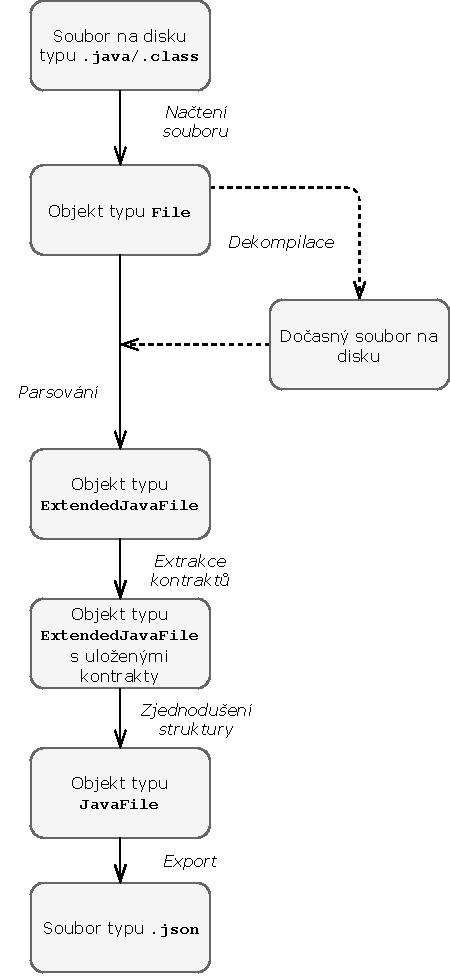
\includegraphics{img/workFlow.pdf}
						\caption[workFlow]{Základní work flow}
						\label{workFlow}
					\endminipage\hfill
				\end{figure}
				
				
%%%%%%%%%%%%%%%%%%%%%%%%%%%%%%%%%%%%%%%%%%%%%%%%%%%%%%%%%%%%%%%%%%%%%%%%%%%%%%%%%%%%%%%%%%%%%%%%%%%%%%%%%%%%%%%%%%%%%%%%%%%%%%%%%%%%%%%%%%%%%%%%%%%%%%%%%%%%%%%%%%%%%%%%%%%%%%%%%%%%%%%%

		\subsection{Parsovací modul}
			Tento modul zajišťuje zpracování zdrojových souborů jazyka Java a následné uložení do reprezentace \texttt{ExtendedJavaFile}. To má na starosti třída \texttt{JavaFileParser}, která také využívá třídy \texttt{MethodVisitor}.\\
			
			Třída \texttt{ExtendedJavaFile} je součástí modelu pro parsování, který dědí od svých rodičovských tříd ze základního datového modelu výše. Dále je zde třída \texttt{ExtendedJavaClass} a \texttt{ExtendedJavaMethod}. Tento rozšířený model ukládá dodatečné informace jako je tělo metod, anotace atd. Z těchto informací jsou následně získávány kontrakty.\\
			
			Vytvořená struktura je následně procházena a jsou z ní extrahovány kontrakty. To zajišťují třídy \texttt{GuavaParser} a \texttt{JSR305Parser} (každá svůj cílený typ kontraktu). Tyto třídy implementují rozhraní \texttt{ContractParser} a továrna \texttt{ParserFactory} umožňuje vytváření jejich instancí. Tímto způsobem se instance objektu \texttt{ExtendedJavaFile} postupně rozšiřuje.\\
			
			Poté co byly extrahovány všechny kontrakty, podrobnosti o metodách a třídách jsou již redundantní a z toho důvodu je objekt \texttt{ExtendedJavaFile} zredukován na \texttt{JavaFile}. Totéž platí pro zbytek modelu. K této redukci slouží třída \texttt{Simplifier}.\\
			
			Poslední částí tohoto modulu je třída \texttt{ContractExtractor}. Ta slouží jako výchozí bod pro komunikaci s ostatními částmi nástroje a spojuje dílčí třídy a jejich funkce dohromady. V podstatě se jedná o API pro vnitřní užití knihovny.\\
			
			Graficky je možné vidět tento modul v podobě UML diagramu, který je zobrazen na obrázku \ref{UMLParser}. Jedná se o zjednodušený UML diagram tříd, kde jsou jednotlivé metody omezeny pouze na svůj název a návratovou hodnotu. Důvodem je to, že metody mají mnoho vstupních parametrů, což by činilo diagram nepřehledný. Podrobnosti o konkrétních třídách je pak možné získat z JavaDoc dokumentace(na CD ve složce \texttt{javaDoc}. Rozšíření model je také zjednodušen a jsou zde zobrazeny pouze atributy, které nemají rodičovské třídy zobrazené v modelu výše.
		
			\subsubsection{Parsování Java souborů}	    
				Pro zpracování zdrojových souborů jazyku Java byla použita knihovna JavaParser. Ta poskytuje metodu \texttt{parse()}, která vytvoří komplexní strukturu daného zdrojového souboru. V prvním kroku se tato struktura projde a vyhledá všechny třídy (\emph{class}) a také rozhraní \emph{interface} a výčtové typy \emph{enum}. Pro účely modelu jsou si tyto tři prvky rovny. Každý nalezený prvek je následně uložen do modelu. V případě třídy a rozhraní se struktura prochází dále a do modelu jsou uloženy všechny konstruktory, které se z hlediska modelu považují za metody (viz níže). Následně jsou uloženy všechny anotace dané \uv{třídy}.\\
			
				Po této přípravě je využita třída \texttt{MethodVisitor}, která dědí od třídy \texttt{VoidVisitorAdapter} a umožňuje procházet všechny metody v daném souboru. V metodě pak máme k dispozici objekt typu \texttt{MethodDeclaration}, který obsahuje všechny potřebné údaje a také rodičovský \texttt{ExtendedJavaFile}. Pro každou metodu je nalezena její rodičovská třída. Hledá se nejvyšší rodič a tudíž vnořené metody nemají jako rodiče vyšší metodu ale nejvyšší dostupnou třídu. Pro danou metodu jsou následně uloženy všechny anotace a i její parametry. Následně je uloženo celé tělo metody jako seznam objektů typu \texttt{Node}, které umožňují další zpracování. Z těchto získaných dat je vytvořena instance objektu \texttt{ExtendedJavaMethod}, která je následně uložena do své rodičovské \texttt{ExtendedJavaClass}.
				
			\subsubsection{Extrakce kontraktů}
			
			\paragraph{Obecně}
				Poté, co je ze Java souboru vytvořen objekt typu \texttt{ExtendedJavaFile}, je možné začít extrahovat kontrakty. Během získávání kontraktů se tato struktura prochází a postupně se k jednotlivým třídám a metodám přidávají kontrakty. Poté, co jsou všechny extrakce dokončeny, je za pomocí třídy \texttt{Simplifier} objekt převeden na typ \texttt{JavaFile}, který obsahuje pouze relevantní informace a je připraven pro export.	Během získávání kontraktů se také postupně aktualizují statistické údaje o počtu kontraktů a o počtu metod, které kontrakty obsahují.	
			
			\paragraph{Guava Precondtions}
				Vzhledem k tomu, že všechny kontrakty tohoto typu jsou realizovány pomocí volání metod ze třídy \texttt{Preconditions}, zaměřuje se extrakce pouze na těla metod a tříd či ostatních částí metod si algoritmus nevšímá. Postupně se procházejí jednotlivé části metody (objekty \texttt{Node}) a ve chvíli kdy se narazí na \texttt{Node}, který je typu \texttt{MethodCallExpr}, tedy jedná se o volání metody, zjišťuje se, zda se jedná o volání některé z metod třídy \texttt{Preconditions}, pokud ano, je tento výraz dále zpracováván. Název Guava metody je uložen do kontraktu jako atribut \texttt{function}. První parametr metody, zpravidla ten klíčový, je uložen jako atribut \texttt{expression}. Ostatní parametry obvykle souvisejí pouze s tvarem chybové zprávy, ty jsou uloženy do seznamu \texttt{arguments}.\\				
				
				Nástroj umožňuje rozpoznání těchto metod: checkArgument, checkState, checkNotNull, checkElementIndex, badElementIndex, checkPositionIndex, badPositionIndex, checkPositionIndexes, badPositionIndexes.\\
				
				Vysvětlení, použití a jiné podrobnosti jednotlivých metod je možné zjistit v dokumentace knihovny. I přesto, že projekt v současné podobě umožňuje rozpoznat všechny metody Guava Preconditions, časem mohou přibýt jiné konstrukce, které bude třeba do nástroje doplnit. Vzhledem k tomu, že Guava je stále živý projekt, který se vyvíjí, je třeba kontrolovat nové verze, zda nepřidávají nové metody pro reprezentaci kontraktů.	
				
			\paragraph{JSR305}
				Na rozdíl od Guava Preconditions mohou být kontrakty typu JSR305 obsaženy v anotacích tříd a metod a také v jejich parametrech. Zde je tedy nutné procházet tyto bloky a naopak těla metod je možné zanedbat. Postupně se procházejí jednotlivé anotace tříd i metod. Jakmile je daná anotace výrazem JSR305, je uložena jako kontrakt. Tvar anotace představuje \texttt{function} a stejně jako v případě Guava, první parametr je uložen jako \texttt{expression} a ostatní jsou uloženy do seznamu \texttt{arguments}. Tyto anotace však obvykle parametr nemají. Takto nalezené kontrakty v anotacích třídy jsou označeny za neměnné proměnné (class invariants) a v anotacích metod se pak jedná o post-conditions, vztahují se k výstupu metody. Zbývají parametry metod, u kterých se opět zkoumají anotace stejným způsobem. Tyto anotace však vždy mívají alespoň jeden atribut a tím je tvar samotného parametru.\\			

				Nástroj umí rozpoznávat následující anotace: CheckForNull, CheckForSigned, CheckReturnValue, Detainted, MatchesPattern, Nonnegative, Nonnull, Nullable, OverridingMethodsMustInvokeSuper, ParametersAreNonnullByDefault, ParametersAreNullableByDefault, PropertyKey, RegEx, Signed, Syntax, Tainted, Untainted, WillClose, WillCloseWhenClosed, WillNotClose.\\
				
				Jedná se o všechny anotace, které má knihovna k dispozici v poslední verzi. Jejich vysvětlení, použití a jiné podrobnosti je možné zjistit v dokumentace knihovny.
			
		

%%%%%%%%%%%%%%%%%%%%%%%%%%%%%%%%%%%%%%%%%%%%%%%%%%%%%%%%%%%%%%%%%%%%%%%%%%%%%%%%%%%%%%%%%%%%%%%%%%%%%%%%%%%%%%%%%%%%%%%%%%%%%%%%%%%%%%%%%%%%%%%%%%%%%%%%%%%%%%%%%%%%%%%%%%%%%%%%%%%%%%%%	
		
		\subsection{Dekompilace Bytcode}
			Jak již bylo zmíněno výše, pro dekompilaci Java \texttt{.class} souborů byla použita knihovna Procyon. Ta poskytuje metodu \texttt{void decompile(String internalName, ITextOutput output)}, která přečte vstupní soubor s přeloženým kódem a do jiného souboru uloží jeho dekompilovanou verzi. V mém nástroji dekompilaci obstarává obalovací metoda \texttt{boolean decompileClass-\\File(String filename)}, která se nachází v třídě \texttt{io.IOServices}. Ta vytvoří dočasný soubor dle konfigurace a vrátí, za byla operace úspěšná. Z hlediska pracovního postupu dekompilaci vyvolává třída \texttt{JavaFileParser} v metodě \texttt{ExtendedJavaFile parseFile(File file)}v případě, že se vstupní soubor má koncovku \texttt{.class}. Pokud je dekompilace bez chyb, je daný, dočasně vytvořený, soubor zpracován stejným způsobem, jako by se jednalo o zdrojový soubor. Po zpracování je dočasný soubor smazán.
					

%%%%%%%%%%%%%%%%%%%%%%%%%%%%%%%%%%%%%%%%%%%%%%%%%%%%%%%%%%%%%%%%%%%%%%%%%%%%%%%%%%%%%%%%%%%%%%%%%%%%%%%%%%%%%%%%%%%%%%%%%%%%%%%%%%%%%%%%%%%%%%%%%%%%%%%%%%%%%%%%%%%%%%%%%%%%%%%%%%%%%%%%
	    


%%%%%%%%%%%%%%%%%%%%%%%%%%%%%%%%%%%%%%%%%%%%%%%%%%%%%%%%%%%%%%%%%%%%%%%%%%%%%%%%%%%%%%%%%%%%%%%%%%%%%%%%%%%%%%%%%%%%%%%%%%%%%%%%%%%%%%%%%%%%%%%%%%%%%%%%%%%%%%%%%%%%%%%%%%%%%%%%%%%%%%%%
		

%%%%%%%%%%%%%%%%%%%%%%%%%%%%%%%%%%%%%%%%%%%%%%%%%%%%%%%%%%%%%%%%%%%%%%%%%%%%%%%%%%%%%%%%%%%%%%%%%%%%%%%%%%%%%%%%%%%%%%%%%%%%%%%%%%%%%%%%%%%%%%%%%%%%%%%%%%%%%%%%%%%%%%%%%%%%%%%%%%%%%%%%	
	    \subsection{Porovnávání kontraktů}
	    	Modul pro porovnávání kontraktů se skládá ze tří tříd a modelu pro porovnávání. Struktura tohoto modulu je vidět na obrázku \ref{comapreModul}. Model byl představen výše (viz 5. kapitola - Datový model) a nebude zde proto opět detailně rozebírán. Dílčími třídami pak jsou \texttt{ContractComparator}, který specifikuje porovnávání samotných kontraktů, \texttt{JavaFileComparator} pro porovnávání souborů a nakonec \texttt{JavaFolderComparator}, který umožňuje porovnávání složek.
	    	
	    \textbf{\textcolor{pblue}{TODO: Přidat detailnější popis + diagram}}\\	


%%%%%%%%%%%%%%%%%%%%%%%%%%%%%%%%%%%%%%%%%%%%%%%%%%%%%%%%%%%%%%%%%%%%%%%%%%%%%%%%%%%%%%%%%%%%%%%%%%%%%%%%%%%%%%%%%%%%%%%%%%%%%%%%%%%%%%%%%%%%%%%%%%%%%%%%%%%%%%%%%%%%%%%%%%%%%%%%%%%%%%%%    
	    \subsection{Popis API}
	    	Knihovna obsahuje API pro snazší přístup zvnějška. Skládá se z několika částí. Je zde třída \texttt{ApiFactory}, která umožňuje instancování jednotlivých API, jedná se o návrhový vzor továrny. V nástroji jsou definovány celkem čtyři různé typy API, každé z nich implementuje specifické rozhraní, pomocí kterého je možné využít továrny. V nástroji je pouze jedna implementace pro každý typ, továrna a rozhraní jsou zde tedy pouze pro přehlednost a možnost snadného rozšíření.\\
	    	
	    	Zde je seznam všech čtyř typů API podle názvů jejich rozhraní. Implementační třídy pak mají stejný název, ale s přidanou předponou \texttt{Default}. Prvním typem je API, které definuje metody pro extrakci kontraktů a jejich export do souborů typu JSON (\texttt{ContractExtractorApi}). Další API typem je \texttt{BatchContractExtractorApi}. Ten umožňuje podobné funkce, s tím rozdílem, že jsou upraveny pro dávkové použití v konzolové části aplikace. Další částí je API pro porovnávání kontraktů (\texttt{ContractComparatorApi}) a opět jeho obdoba pro dávkové zpracování (BatchContractComparatorApi). Následuje stručný výčet toho, co jednotlivá API umožňují. Pro přesný popis metod, jejich parametrů a návratového typu je možné se podívat do JavaDoc projektu.
	    
			\subsubsection{ContractExtractorApi}
					Zde jsou zejména metody pro získání kontraktů. Metoda \texttt{retrieveContracts} umožňuje extrakci kontraktů ze vstupního souboru. Je možné definovat, které typy kontraktů se mají získat a zda mají být vráceny i objekty bez kontraktů. Vrácena je instance \texttt{JavaFile}, která obsahuje extrahované kontrakty. Další metodou je \texttt{retrieveContractsFromFolder}, která poskytuje stejnou funkcionalitu s tím rozdílem že vstupem je celá složka nikoliv soubor a je vrácen seznam \texttt{JavaFile}.\\
					
					Následně je zde \texttt{exportJavaFilesToJson}. Tato metoda slouží k exportu vstupního seznamu \texttt{JavaFile} do JSON. Je třeba nastavit výstupní složku a také zda má být formát v minimalistické formě. Poslední metodou pak je \texttt{updateShortPathOfJavaFiles}, která aktualizuje atribut \texttt{shortPath} všech \texttt{JavaFile} v seznamu.	    
			    
			\subsubsection{BatchContractExtractorApi}	
				Toto API poskytuje podobnou funkcionalitu jako předchozí. Obsahuje pouze jednu metodu \texttt{retrieveContractsFromFolderExportToJson}. Jedná se v podstatně o kombinaci předchozích metod. Umožňuje načtení kontraktů z dané složky a jejich následný export do zadaného adresáře, součástí je také shodné nastavení. Tato metoda nejprve načte jeden soubor ten zpracuje, exportuje a pak pokračuje dalším, díky tomu je méně náročná na paměť.
				
			\subsubsection{ContractComparatorApi}
				Poskytuje metodu \texttt{compareJavaFolders}, která porovná dvě zadané složky na úrovni jejich API a kontraktů a vytvoří report \texttt{JavaFolderCompareReport}. Je možné zvolit, zda se mají reportovat shodné objekty a také jestli se mají reportovat změny, které přímo neovlivňují kontrakty. Druhou metodou je pak \texttt{exportJavaFolderCompareReportToJson}, což umožňuje vytvořený report exportovat do JSON.
				
			\subsubsection{BatchContractComparatorApi}
				Toto je poslední dostupné API. Opět poskytuje obdobné chování jako předchozí API, s tím rozdílem, že je určeno pro dávkové zpracování a kombinuje obě metody do jedné(\texttt{compareJavaFoldersAndExportToJson}). Tato metoda porovná obě složky a výslednou zprávu následně exportuje do JSON.
				
			\subsubsection{Použití API}	    
				Použití API je velmi snadné jak je vidět na příkladu níže.\\\\
				\- \- \- \- \- \- \texttt{\textcolor{pgrey}{// Získání instance API pomocí továrny}}\\ 
				\- \- \- \- \- \- \texttt{ApiFactory f = new ApiFactory();}\\
	    		\- \- \- \- \- \- \texttt{ContractExtractorApi api = f.getContractExtractorApi();}\\  
            	\- \- \- \- \- \- \texttt{\textcolor{pgrey}{// Nyní je možné využít metody knihovny}}\\ 
				\- \- \- \- \- \- \texttt{api.retrieveContracts(...);}\\
	    
%%%%%%%%%%%%%%%%%%%%%%%%%%%%%%%%%%%%%%%%%%%%%%%%%%%%%%%%%%%%%%%%%%%%%%%%%%%%%%%%%%%%%%%%%%%%%%%%%%%%%%%%%%%%%%%%%%%%%%%%%%%%%%%%%%%%%%%%%%%%%%%%%%%%%%%%%%%%%%%%%%%%%%%%%%%%%%%%%%%%%%%%
	    \subsection{Přidání parseru pro nový typ kontraktu}
	    	Při vytváření knihovny i aplikace byl kladen důraz na abstrakci od použitých typů kontraktů, aby bylo možné snadno přidat parser pro nový typ kontraktu. Grafickou aplikaci není třeba nijak měnit, ale je třeba provést několik kroků v rámci knihovny. Pro rozpoznávání nové reprezentace kontraktu jsou potřeba tyto kroky:
	    	
			\begin{enumerate}
				\item Přidání položky do \texttt{ContractType}
				\item Vytvoření nového analyzátoru
				\item Doplnění továrny \texttt{ParserFactory}
				\item Testování
			\end{enumerate}				    	
	    	
	    	\subsubsection{Přidání položky do \texttt{ContractType}}
	    		Nejprve je třeba přidat položku do výčtového typu \texttt{ContractType}. Název by měl být vhodně zvolen, protože je zobrazen v exportovaných datech, ale i v grafické aplikaci. Kontext je dobře vidět na diagramu datového modelu (obrázek \ref{modelExtractorDiagram} v předchozí kapitole).
	    		
	    	\subsubsection{Vytvoření nového analyzátoru}
	    		Následně je třeba vytvořit funkční část daného parseru. Je tedy nutné vytvořit třídu, která bude implementovat rozhraní \texttt{ContractParser}. Toto rozhraní požaduje implementaci pouze jedné metody a tou je \texttt{ExtendedJavaFile retrieveContracts(ExtendedJavaFile extendedJavaFile)}. Aby byly zachovány jmenné konvence současné knihovny, měla by se tato třída jmenovat \texttt{TypXParser}, kde \texttt{TypX} reprezentuje název nového typu kontraktu. Tato třída by se měla nacházet v balíčku se stejným jménem (ale s malými písmeny) a ten by se měl nacházet v balíčku \texttt{cz.zcu.kiv.contractparser.parser}. Tvar samotné metody již závisí na principech daného kontraktu. Obecně platí, že by se měly kontrakty detekovat a vytvořit na základě dat ze vstupního objektu typu \texttt{ExtendedJavaFile} a ve stejném objektu je také vrátit. Pro lepší představu doporučuji prozkoumat již implementované analyzátory pro JSR305 a Guava Preconditions.
	    		
	    	\subsubsection{Doplnění továrny \texttt{ParserFactory}} 
	    		Dalším krokem je doplnění továrny \texttt{ParserFactory}. Zde je pouze třeba přidat nový \texttt{case} do konstrukce \texttt{switch}. Tento blok by měl vracet instanci nového parseru v případě že vstoupí tento typ v objektu \texttt{ContractType}.
	    			
	    	\subsubsection{Testování}
	    		Pro bezchybnou funkci daného analyzátoru je vhodné vytvoření testů. Testovací data pro současné testy jsou umístěny v \texttt{resources/testFiles}, kde jsou pak dále děleny do složek.

    
    
    
    
%%%%%%%%%%%%%%%%%%%%%%%%%%%%%%%%%%%%%%%%%%%%%%%%%%%%%%%%%%%%%%%%%%%%%%%%%%%%%%%%%%%%%%%%%%%%%%%%%%%%%%%%%%%%%%%%%%%%%%%%%%%%%%%%%%%%%%%%%%%%%%%%%%%%%%%%%%%%%%%%%%%%%%%%%%%%%%%%%%%%%%%%
%%%%%%%%%%%%%%%%%%%%%%%%%%%%%%%%%%%%%%%%%%%%%%%%%%%%%%%%%%%%%%%%%%%%%%%%%%%%%%%%%%%%%%%%%%%%%%%%%%%%%%%%%%%%%%%%%%%%%%%%%%%%%%%%%%%%%%%%%%%%%%%%%%%%%%%%%%%%%%%%%%%%%%%%%%%%%%%%%%%%%%%%
%%%%%%%%%%%%%%%%%%%%%%%%%%%%%%%%%%%%%%%%%%%%%%%%%%%%%%%%%%%%%%%%%%%%%%%%%%%%%%%%%%%%%%%%%%%%%%%%%%%%%%%%%%%%%%%%%%%%%%%%%%%%%%%%%%%%%%%%%%%%%%%%%%%%%%%%%%%%%%%%%%%%%%%%%%%%%%%%%%%%%%%%
%%%%%%%%%%%%%%%%%%%%%%%%%%%%%%%%%%%%%%%%%%%%%%%%%%%%%%%%%%%%%%%%%%%%%%%%%%%%%%%%%%%%%%%%%%%%%%%%%%%%%%%%%%%%%%%%%%%%%%%%%%%%%%%%%%%%%%%%%%%%%%%%%%%%%%%%%%%%%%%%%%%%%%%%%%%%%%%%%%%%%%%%
	\section{Uživatelská aplikace}
	   \subsection{Použité technologie}
	    	 Aplikace byla, stejně jako knihovna, implementována v jazyce Java verze 1.8 ve vývojovém prostředí IDEA IntelliJ Ultimate 2017.3.3 s využitím Apache Maven. Grafické uživatelské rozhraní bylo vytvořeno využitím platformy JavaFX. 
	    	 
	    	 \subsubsection{Externí knihovny}
				Mimo následujících knihoven byly opět využity externí knihovny Apache Log4j a Google Gson, které byly popsány výše.
			
			\paragraph{ControlsFX} 
				Tato knihovna rozšiřuje JavaFX a umožňuje použití dalších funkcí a objektů zejména pak \texttt{CheckListView}, což je použito pro zobrazení seznamu souborů \cite{controlsfx}. 
			
			\paragraph{FontAwesomeFX} 	
				Knihovna FontAwesomeFX slouží opět k rozšíření JavaFX. Tuto knihovnu jsem použil pro rozšíření možností zobrazení ikon \cite{fontawesomefx}.	 
		
		\subsection{Struktura aplikace}
			\textbf{\textcolor{pblue}{TODO: }}\\		
		
	    	   
	   \subsection{Ovládání aplikace}
	   		Pro zlepšení práce s aplikací, byla rozdělena na dvě části. Aplikaci je možné spustit bez parametrů jako grafickou aplikaci, případně je možné aplikaci spustit s parametry, čímž se provede jednorázová akce pro dávkové zpracování. Podrobné informace o spouštění a používání aplikace jsou uvedeny v příloze A. Uživatelská příručka.
	   		
	   		\subsubsection{Grafická část}
	   			Standardním spuštěním aplikace bez parametrů se zobrazí grafická uživatelská část. Zde je možné extrahovat kontrakty, zobrazovat si je v kontextu hierarchie daného souboru, exportovat získaná data a také porovnávat složky za účelem zjištění rozdílů v API a kontraktech. Všechny tyto činnosti je možné obsluhovat pomocí jednoduchého a intuitivního uživatelského rozhraní.			   			  		
	   		\subsubsection{Konzolová část}
	   			V případě, že chceme pouze provést jednorázovou akci extrakce či porovnávání kontraktů a následný export, je možné využít konzolové části aplikace, tedy spustit aplikaci s příslušnými parametry (viz Uživatelská příručka). Takto je možné snadno a rychle provádět dávkové operace. Tento způsob zpracování je také méně náročný na paměť zařízení.
	   
	   \subsection{Možnosti a limitace aplikace}
	   		Při vývoji uživatelské aplikace byl kladen důraz na snadné a intuitivní použití, které poskytne možnost jak vyzkoušet a aktivně využít vytvořenou knihovnu. Nástroj je určen pro výzkumné účely uzavřené skupiny, nikoliv pro použití širší veřejností. Z tohoto důvodu nebyl kladen důraz na její široké možnosti a uživateli může připadat, že postrádá prvky, které jsou typické pro komerční aplikace. Příkladem může být perzistence dat, široké možnosti filtrování a řazení, propojení s externími editory atd. Níže, v podkapitole Prostor pro zlepšení, je této problematice věnována větší část.




%%%%%%%%%%%%%%%%%%%%%%%%%%%%%%%%%%%%%%%%%%%%%%%%%%%%%%%%%%%%%%%%%%%%%%%%%%%%%%%%%%%%%%%%%%%%%%%%%%%%%%%%%%%%%%%%%%%%%%%%%%%%%%%%%%%%%%%%%%%%%%%%%%%%%%%%%%%%%%%%%%%%%%%%%%%%%%%%%%%%%%%%
%%%%%%%%%%%%%%%%%%%%%%%%%%%%%%%%%%%%%%%%%%%%%%%%%%%%%%%%%%%%%%%%%%%%%%%%%%%%%%%%%%%%%%%%%%%%%%%%%%%%%%%%%%%%%%%%%%%%%%%%%%%%%%%%%%%%%%%%%%%%%%%%%%%%%%%%%%%%%%%%%%%%%%%%%%%%%%%%%%%%%%%%
%%%%%%%%%%%%%%%%%%%%%%%%%%%%%%%%%%%%%%%%%%%%%%%%%%%%%%%%%%%%%%%%%%%%%%%%%%%%%%%%%%%%%%%%%%%%%%%%%%%%%%%%%%%%%%%%%%%%%%%%%%%%%%%%%%%%%%%%%%%%%%%%%%%%%%%%%%%%%%%%%%%%%%%%%%%%%%%%%%%%%%%%
%%%%%%%%%%%%%%%%%%%%%%%%%%%%%%%%%%%%%%%%%%%%%%%%%%%%%%%%%%%%%%%%%%%%%%%%%%%%%%%%%%%%%%%%%%%%%%%%%%%%%%%%%%%%%%%%%%%%%%%%%%%%%%%%%%%%%%%%%%%%%%%%%%%%%%%%%%%%%%%%%%%%%%%%%%%%%%%%%%%%%%%%	   
\section{Optimalizace}

	obecně, snažil jsem se zajistit co nejlepší...

 \subsection{Analýza a refaktoring kódu}
  	- ručně, nástroje IDE, -> snížení cyklomatičnosti, zpřehlednění kódu
  	
 \subsection{Zjdenodušení modelu} 
 	- vyhnutí se použití rozsáhlých obejktů knihovny
 	- pozitivní dopad na paměťovou náročnost, zpřehlednění modelu

 - při batch soubory průběžně ukládat, aby nezatěžovalo paměť
 - přeparsování souborů se nevyplatí - stačí udělat vše a pak jen filtrovat 
 - rozebrat nároky na paměť v aplikaci


% Optimalizace
\chapter{Optimalizace}
 - Analýza a refaktoring kódu (snížení cyklomatičnosti)
 - Zjdenodušení modelu - vyhnutí se použití rozsáhlých obejktů knihovny
 - při batch soubory průběžně ukládat, aby nezatěžovalo paměť
 - přeparsování souborů se nevyplatí - stačí udělat vše a pak jen filtrovat 
 - rozebrat nároky na paměť v aplikaci


% Testování
\chapter{Testování}
 - Unit testy 
 - integrační testy - malá aplikace nemusí se tolik řešit
 - funkční testy - testovat na úrovni GUI (ošetření vstupů)
 - popis testovacích dat (syntetická, skutečná - výsledky testů)
 - PMD

% Zhodnocení výsledků
\chapter{Zhodnocení výsledků}
	Hlavní cíle této práce byl úspěšně zapracovány. Ze vstupních souborů je možné extrahovat konstrukce DbC, které je možné dále exportovat do vnější reprezentace či porovnávat. Funkcionalita tohoto nástroje je pak zakomponována do uživatelské aplikace. Řešení má samozřejmě své silné i slabé stránky a zde bude proveden jejich rozbor.	
	
	
	\section{Úspěšnost detekce kontraktů}
		Na základě provedených testů a analýzy se mi podařilo úspěšně detekovat všechny kontrakty typu JSR305 či Guava Preconditions. Tyto kontrakty byly úspěšně uloženy do navržené datové struktury připraveny pro další zpracování. Kontrakty je možné extrahovat ze zdrojových i přeložených souborů jazyka Java. Kód daného souboru však musí být validní, jinak není možné jej zpracovat analyzátorem.
	
	\section{Úspěšnost porovnání kontraktů}
		\textbf{\textcolor{pblue}{TODO: Doplnit dle implementace porovnávání kontraktů}}
	 	
 	\section{Prostor pro zlepšení}

		\subsection{Rozpoznání dalších kontraktů}
			Nástroj momentálně umožňuje rozpoznání pouze dvou typů kontraktů (JSR305, Guava Preconditions). To je pro použití v praxi samozřejmě nedostačující a dalším logickým krokem ve vývoji by mělo být přidání rozpoznání dalších specifikací. Nástroj je na to připraven a z hlediska integrace by se tedy nemělo jednat o problém. Obtížnost samotného rozpoznání je pak závislá na povaze dané reprezentace.
			
		\subsection{Porovnávání}
			Pro porovnávání dvou složek se soubory obsahujícími kontrakty je možné udělat pokročilejší párování souborů. Pokud je soubor pouze přejmenován či přesunut je to kvalifikováno, jako že byl soubor odstraněn, respektive přidán, díky čemuž dané dva soubory nejsou porovnány. Pro částečné odstranění tohoto problému by bylo možné vytvořit heuristiku, která by porovnávala obsahy souborů, případně by bylo možné dát uživateli volbu v případě neprůkaznosti.\\
			
			\textbf{\textcolor{pblue}{TODO: Doplnit dle implementace porovnávání kontraktů}}
  		
  		\subsection{Efektivita}
	  		Aplikace poskytuje prostor pro zlepšení v rámci efektivity algoritmů. Činnosti jako extrakce či porovnání by mohly být zpracovávány paralelně, což by mohlo činnost značně urychlit. V současné době se jednotlivé kontraktů zpracovávají sekvenčně, nicméně při snaze zvýšit efektivitu by bylo možné tyto činnosti spojit dohromady a snížit tak cyklomatičnost celého procesu. Toto zlepšení by však bylo na úkor přehlednosti, jelikož by se museli jednotlivé algoritmy prolínat.\\
  		
  		\subsection{Uživatelská aplikace}
  			Vzhledem k tomu, že bylo cílem vytvořit pouze jednoduchou uživatelskou aplikaci, která bude primárně sloužit pro další výzkum této problematiky, je v této oblasti mnoho prostoru pro zlepšení. V současné podobně je aplikace vhodná pro zpracování menšího či středního množství souborů. Pro rozšířené použití, by bylo nasnadě zlepšit zobrazení souborů, které by bylo možné např. členit dle projektů, ukládat či jinak zachovávat současné projekty a obecně přidání funkcionalit tohoto typu.\\ 
  			
  			S těmito rozšířeními pro zpracování souborů by také souviselo perzistence zpracovaných dat. Momentálně jsou zpracované soubory uchovávány v paměti, což při malém množství souborů zrychluje práci, nicméně při větším množství souborů se jedná o paměťově náročnou činnost. Zpracované soubory by se tak mohli ukládat např. na pevný disk či do databáze.\\
  			
  			Pro zlepšení celkové uživatelské zkušenosti by také bylo vhodné doplnit řadu dodatečných akcí, které jsou typické pro programy na správu dat, jak je např. řazení souborů, další možnosti filtrace, ale např. také umožnit použití klávesových zkratek.\\
  			
  			V případě potřeby by také bylo možné zdokonalit konzolovou část aplikace, která by mohla poskytovat dodatečnou funkcionalitu či nastavení.\\
  			
  			Myslím, že díky své silně technické a akademické povaze, není potřebné žádné vylepší vzhledu, které by mohlo být prospěšné např. u komerční aplikace.

% Závěr
\chapter{Závěr}
	\textbf{\textcolor{pblue}{TODO: Doplnit}}\\

% Přehled zkratek
\chapter*{Přehled zkratek a použitých výrazů}
\textbf{\textcolor{pblue}{TODO: Doplnit}}\\
\paragraph{DbC}
Design By Contract



% Literatura
\begin{thebibliography}{99}

%%%%%%%%%%%%%%%%%%%%%%%%%%%%%%%%%%%%%%%%%%%%%%%%%%%%%%%%%%%%%%%%%%%%%%%%%%%%%%%%%%%%%%%%%%%%%%%%%%%%%%%%%%%%%%%%%%%%%%%%%%%%%%%%%%%%%%%%%%%%%%%%%%%%%%%%%%%%%%%%%%%%%%%%%%%%%%%%%%%%%%%%%%%%%%%%%%%%%%%
%%%%%%%%%%%%%%%%%%%%%%%%%%%%%%%%%%%%%%%%%%%%%%%%%%%%%%%%%%%%%%%%%%%%%%%%%%%%%%%%%%%%%%%%%%%%%%%%%%%%%%%%%%%%%%%%%%%%%%%%%%%%%%%%%%%%%%%%%%%%%%%%%%%%%%%%%%%%%%%%%%%%%%%%%%%%%%%%%%%%%%%%%%%%%%%%%%%%%%%
% Zajištění kvality software
\bibitem{swqa} Dr. Ulbert Zsolt:\emph{Software Development Process and Software Quality Assurance}. University of Pannonia 2014

\bibitem{defProgram} {\it Defensive Programming} [online]. [cit. 2018-05-22]. \textless\url{drdobbs.com/defensive-programming/184401915}\textgreater

\bibitem{misra} {\it MISRA} [online]. [cit. 2018-06-03]. \textless\url{misra.org.uk}\textgreater


%%%%%%%%%%%%%%%%%%%%%%%%%%%%%%%%%%%%%%%%%%%%%%%%%%%%%%%%%%%%%%%%%%%%%%%%%%%%%%%%%%%%%%%%%%%%%%%%%%%%%%%%%%%%%%%%%%%%%%%%%%%%%%%%%%%%%%%%%%%%%%%%%%%%%%%%%%%%%%%%%%%%%%%%%%%%%%%%%%%%%%%%%%%%%%%%%%%%%%%
%%%%%%%%%%%%%%%%%%%%%%%%%%%%%%%%%%%%%%%%%%%%%%%%%%%%%%%%%%%%%%%%%%%%%%%%%%%%%%%%%%%%%%%%%%%%%%%%%%%%%%%%%%%%%%%%%%%%%%%%%%%%%%%%%%%%%%%%%%%%%%%%%%%%%%%%%%%%%%%%%%%%%%%%%%%%%%%%%%%%%%%%%%%%%%%%%%%%%%%
% Popis kontraktů softwarových rozhraní
\bibitem{contractsInWild} Jens Dietrich, David J. Pearce, Kamil Jezek, and Premek Brada:\emph{Contracts in the Wild: A~Study of Java Programs}. In LIPIcs-Leibniz International Proceedings in Informatics (Vol. 74), ECOOP 2017. Schloss Dagstuhl-Leibniz-Zentrum fuer Informatik. 2017

\bibitem{applyingDbc} Bertrand Meyer, “Applying ’design by contract’,” Computer, vol. 25, no. 10, pp. 40–51, Oct 1992

\bibitem{ooswConstruction} Bertrand Meyer, Object-oriented software construction, Prentice-Hall international series in computer science, 1988 

\bibitem{contractAware} Antoine Beugnard, Jean-Marc Jézéquel, Noël Plouzeau, and Damien Watkins. Making Components Contract Aware. Computer, 32(7):38–45, 1999

%\bibitem{designByContractComponentware} Andreas Rausch:\emph{"Design by Contract" + "Componentware" = "Design by Signed Contract"}. Journal of Object Technology 2002, Vol. 1 Pages 20-36 

% Bertrand Meyer
\bibitem{meyerBio} {\it Bertrand Meyer's technology + blog} [online]. [cit. 2018-04-11]. \textless\url{bertrandmeyer.com/bio/}\textgreater
\bibitem{eiffelStudio} {\it EiffelStudio} [online]. [cit. 2018-04-13]. \textless\url{dev.eiffel.com}\textgreater

% Kontrakty v jazyce Java
\bibitem{guava} {\it Guava Preconditions} [online]. [cit. 2018-04-21]. \textless\url{github.com/google/guava}\textgreater
\bibitem{guavaTutorial} {\it tutorialspoint - Guava Preconditions} [online]. [cit. 2018-06-15]. \textless\url{https://www.tutorialspoint.com/guava/guava_preconditions_class.htm}\textgreater
\bibitem{jsr305} {\it JSR305} [online]. [cit. 2018-04-21]. \textless\url{jcp.org/en/jsr/detail?id=305}\textgreater
\bibitem{cofoja} {\it Cofoja} [online]. [cit. 2018-04-21]. \textless\url{github.com/nhatminhle/cofoja}
\bibitem{valid4j} {\it valid4j} [online]. [cit. 2018-04-21]. \textless\url{valid4j.org}	
\bibitem{jcontractor} {\it jContractor} [online]. [cit. 2018-04-22]. \textless\url{jcontractor.sourceforge.net}

% Kontrakty v ostatních technologiích
\bibitem{codeContracts} {\it Code Contracts} [online]. [cit. 2018-04-22]. \textless\url{microsoft.com/en-us/research/project/code-contracts/}\textgreater
\bibitem{codeContracts2} {\it Dokumentace Code Contracts} [online]. [cit. 2018-04-22]. \textless\url{docs.microsoft.com/en-us/dotnet/framework/debug-trace-profile/code-contracts}\textgreater
\bibitem{phpDeal} {\it PhpDeal} [online]. [cit. 2018-04-22]. \textless\url{github.com/php-deal/framework}\textgreater
\bibitem{boostContract} {\it Boost.Contract} [online]. [cit. 2018-04-22]. \textless\url{boost.org/doc/libs/master/libs/contract}\textgreater
\bibitem{eiffel} {\it Eiffel} [online]. [cit. 2018-04-22]. \textless\url{eiffel.org}\textgreater

% Java
\bibitem{javaEnviroment} {\it The Java Language Environment} [online]. [cit. 2018-05-01]. \textless\url{oracle.com/technetwork/java/langenv-140151.html}\textgreater
\bibitem{javaTrend} {\it TIOBE Trend of programming languages} [online]. [cit. 2018-05-01]. \textless\url{tiobe.com/tiobe-index}\textgreater
\bibitem{compilerTutorial} {\it Compiler Design Tutorial} [online]. [cit. 2018-05-01]. \textless\url{tutorialspoint.com/compiler_design}\textgreater
\bibitem{jit} {\it Just-In-Time Compilers} [online]. [cit. 2018-05-01]. \textless\url{webbasedprogramming.com/Java-Unleashed-Second-Edition/ch44.htm}\textgreater
\bibitem{classLoad} {\it Internals of Java Class Loading} [online]. [cit. 2018-05-01]. \textless\url{onjava.com/pub/a/onjava/2005/01/26/classloading.html}\textgreater

% Parsery
\bibitem{jflex} {\it JFlex} [online]. [cit. 2018-05-01]. \textless\url{jflex.de}\textgreater
\bibitem{antlr} {\it ANTLR} [online]. [cit. 2018-05-01]. \textless\url{antlr.org}\textgreater
\bibitem{javaparser} {\it JavaParser} [online]. [cit. 2018-05-01]. \textless\url{javaparser.org}\textgreater
\bibitem{roaster} {\it Roaster} [online]. [cit. 2018-05-01]. \textless\url{github.com/forge/roaster}\textgreater




% Dekompilátory
\bibitem{top8decompilers} {\it Top 8 Java Decompilers} [online]. [cit. 2018-05-02]. \textless\url{crunchytricks.com/2016/07/best-offline-java-decompilers.html}\textgreater
\bibitem{decompilersOnline} {\it Decompilers Online} [online]. [cit. 2018-05-02]. \textless\url{javadecompilers.com}\textgreater
\bibitem{quickDecompilers} {\it A Quick Look at Java Decompilers} [online]. [cit. 2018-05-02]. \textless\url{blog.macuyiko.com/post/2015/a-quick-look-at-java-decompilers.html}\textgreater

\bibitem{jd} {\it JD Project} [online]. [cit. 2018-05-02]. \textless\url{jd.benow.ca}\textgreater
\bibitem{procyon} {\it Procyon} [online]. [cit. 2018-05-02]. \textless\url{bitbucket.org/mstrobel/procyon}\textgreater
\bibitem{cfr} {\it CFR} [online]. [cit. 2018-05-02]. \textless\url{benf.org/other/cfr}\textgreater

%%%%%%%%%%%%%%%%%%%%%%%%%%%%%%%%%%%%%%%%%%%%%%%%%%%%%%%%%%%%%%%%%%%%%%%%%%%%%%%%%%%%%%%%%%%%%%%%%%%%%%%%%%%%%%%%%%%%%%%%%%%%%%%%%%%%%%%%%%%%%%%%%%%%%%%%%%%%%%%%%%%%%%%%%%%%%%%%%%%%%%%%%%%%%%%%%%%%%%
%%%%%%%%%%%%%%%%%%%%%%%%%%%%%%%%%%%%%%%%%%%%%%%%%%%%%%%%%%%%%%%%%%%%%%%%%%%%%%%%%%%%%%%%%%%%%%%%%%%%%%%%%%%%%%%%%%%%%%%%%%%%%%%%%%%%%%%%%%%%%%%%%%%%%%%%%%%%%%%%%%%%%%%%%%%%%%%%%%%%%%%%%%%%%%%%%%%%%%

\bibitem{jsonSyntax} {\it W3Schools - JSON Sytnax} [online]. [cit. 2018-16-06]. \textless\url{https://www.w3schools.com/js/js_json_syntax.asp}\textgreater
	

% Knihovny
\bibitem{maven} {\it Apache Maven} [online]. [cit. 2018-05-05]. \textless\url{maven.apache.org}\textgreater
\bibitem{log4j} {\it Apache Log4j} [online]. [cit. 2018-04-11]. \textless\url{logging.apache.org/log4j/2.x/download.html}\textgreater
\bibitem{gson} {\it Gson} [online]. [cit. 2018-04-11]. \textless\url{github.com/google/gson}\textgreater
\bibitem{junit} {\it jUnit} [online]. [cit. 2018-04-11]. \textless\url{junit.org/junit5/}\textgreater
\bibitem{controlsfx} {\it ControlsFX} [online]. [cit. 2018-04-12]. \textless\url{fxexperience.com/controlsfx/}\textgreater
\bibitem{fontawesomefx} {\it FontAwesomeFX} [online]. [cit. 2018-04-12]. \textless\url{bitbucket.org/Jerady/fontawesomefx}\textgreater




\end{thebibliography}


% Seznam příloh
\chapter*{Seznam příloh}

A Uživatelská příručka
B Obsah CD

\appendix

% A Uživatelská příručka
\chapter{Uživatelská příručka}
	\textbf{\textcolor{pblue}{TODO: Doplnit}}\\

% B Obsah CD
\chapter{Obsah CD}
	Přiložené CD je členěno následujícím způsobem: Je zde složka \texttt{bin}, ve které se nachází spustitelný soubor \texttt{ContractManager.jar}, který slouží ke spuštění uživatelské aplikace. Dále je zde složka \texttt{document}, ve které se nachází tento dokument ve formátu pdf (\texttt{vmares\_dp.pdf}) spolu se zdrojovými soubory, které se nachází ve složce \texttt{src}. Práce byla vytvořena pomocí sázecího software LaTeX.\\
	
	Adresář \texttt{poster} obsahuje poster k diplomové práci ve formátu \texttt{.pub} a \texttt{pdf}. Poslední složkou je pak \texttt{src}, která obsahuje adresáře \texttt{ContractParser} a \texttt{ContractManager}. Tyto složky obsahují zdrojové kódy pro knihovnu a uživatelskou aplikace vytvořeného nástroje.\\
	
	Na CD se také nachází soubor \texttt{readme.txt}, který také obsahuje popis adresářové struktury. Grafické znázornění adresářové struktury je možné vidět níže.

	\subsubsection{Adresářová struktura}
	\noindent
	\texttt{|----- \textbf{bin}}\\
	\texttt{|\- \- \- \- |----- ContractManager.jar}\\
	\texttt{|}\\
	\texttt{|----- \textbf{document}}\\
	\texttt{|\- \- \- \- |----- \textbf{src}}\\
	\texttt{|\- \- \- \- |----- vmares\_dp.pdf}\\
	\texttt{|}\\
	\texttt{|----- \textbf{poster}}\\
	\texttt{|}\\
	\texttt{|----- \textbf{src}}\\
	\texttt{|\- \- \- \- |----- \textbf{ContractManager}}\\
	\texttt{|\- \- \- \- |----- \textbf{ContractParser}}\\
	\texttt{|}\\
	\texttt{|----- readme.txt}\\

\end{document}